%&preformat-synopsis
\RequirePackage[l2tabu,orthodox]{nag} % Раскомментировав, можно в логе получать рекомендации относительно правильного использования пакетов и предупреждения об устаревших и нерекомендуемых пакетах

% Откомментируйте, чтобы отключить генерацию закладок в pdf
% \PassOptionsToPackage{bookmarks=false}{hyperref}
%\documentclass[a5paper,10pt,twoside,openany,article]{memoir} %,draft
\documentclass[a4paper,14pt,oneside,openany]{memoir}


%%%%%%%%%%%%%%%%%%%%%%%%%%%%%%%%%%%%%%%%%%%%%%%%%%%%%%%%%%%%%%%%%%%%%%%%%%%%%%%%
%%%% Файл упрощённых настроек шаблона, общих для диссертации и автореферата %%%%
%%%%%%%%%%%%%%%%%%%%%%%%%%%%%%%%%%%%%%%%%%%%%%%%%%%%%%%%%%%%%%%%%%%%%%%%%%%%%%%%

%%% Режим черновика %%%
\makeatletter
\@ifundefined{c@draft}{
  \newcounter{draft}
  \setcounter{draft}{0}  % 0 --- чистовик (максимальное соблюдение ГОСТ)
                         % 1 --- черновик (отклонения от ГОСТ, но быстрая
                         %       сборка итоговых PDF)
}{}
\makeatother

%%% Пометки в тексте %%%
\makeatletter
\@ifundefined{c@showmarkup}{
  \newcounter{showmarkup}
  \setcounter{showmarkup}{0}  % 0 --- скрыть пометки
                              % 1 --- показывать пометки
}{}
\makeatother

%%% Использование в pdflatex шрифтов не по-умолчанию %%%
\makeatletter
\@ifundefined{c@usealtfont}{
  \newcounter{usealtfont}
  \setcounter{usealtfont}{1}    % 0 --- шрифты на базе Computer Modern
                                % 1 --- использовать пакет pscyr, при его
                                %       наличии
                                % 2 --- использовать пакет XCharter, при наличии
                                %       подходящей версии
}{}
\makeatother

%%% Использование в xelatex и lualatex семейств шрифтов %%%
\makeatletter
\@ifundefined{c@fontfamily}{
  \newcounter{fontfamily}
  \setcounter{fontfamily}{1}  % 0 --- CMU семейство. Используется как fallback;
                              % 1 --- Шрифты от MS (Times New Roman и компания)
                              % 2 --- Семейство Liberation
}{}
\makeatother

%%% Библиография %%%
\makeatletter
\@ifundefined{c@bibliosel}{
  \newcounter{bibliosel}
  \setcounter{bibliosel}{1}   % 0 --- встроенная реализация с загрузкой файла
                              %       через движок bibtex8;
                              % 1 --- реализация пакетом biblatex через движок
                              %       biber
}{}
\makeatother

%%% Вывод типов ссылок в библиографии %%%
\makeatletter
\@ifundefined{c@mediadisplay}{
  \newcounter{mediadisplay}
  \setcounter{mediadisplay}{2}   % 0 --- не делать ничего; надписи [Текст] и
                                 %       [Эл. ресурс] будут выводиться только в ссылках с
                                 %       заполненным полем `media`;
                                 % 1 --- автоматически добавлять надпись [Текст] к ссылкам с
                                 %       незаполненным полем `media`; таким образом, у всех
                                 %       источников будет указан тип, что соответствует
                                 %       требованиям ГОСТ
                                 % 2 --- автоматически удалять надписи [Текст], [Эл. Ресурс] и др.;
                                 %       не соответствует ГОСТ
                                 % 3 --- автоматически удалять надпись [Текст];
                                 %       не соответствует ГОСТ
                                 % 4 --- автоматически удалять надпись [Эл. Ресурс];
                                 %       не соответствует ГОСТ
}{}
\makeatother

%%% Предкомпиляция tikz рисунков для ускорения работы %%%
\makeatletter
\@ifundefined{c@imgprecompile}{
  \newcounter{imgprecompile}
  \setcounter{imgprecompile}{0}   % 0 --- без предкомпиляции;
                                  % 1 --- пользоваться предварительно
                                  %       скомпилированными pdf вместо генерации
                                  %       заново из tikz
}{}
\makeatother
          % общие настройки шаблона
%%% Проверка используемого TeX-движка %%%
\newif\ifxetexorluatex   % определяем новый условный оператор (http://tex.stackexchange.com/a/47579)
\ifxetex
    \xetexorluatextrue
\else
    \ifluatex
        \xetexorluatextrue
    \else
        \xetexorluatexfalse
    \fi
\fi

\newif\ifsynopsis           % Условие, проверяющее, что документ --- автореферат

\usepackage{etoolbox}[2015/08/02]   % Для продвинутой проверки разных условий
\providebool{presentation}

\usepackage{comment}    % Позволяет убирать блоки текста (добавляет
                        % окружение comment и команду \excludecomment)

%%% Поля и разметка страницы %%%
\usepackage{pdflscape}  % Для включения альбомных страниц
\usepackage{geometry}   % Для последующего задания полей

%%% Математические пакеты %%%
\usepackage{amsthm,amsmath,amscd}   % Математические дополнения от AMS
\usepackage{amsfonts,amssymb}       % Математические дополнения от AMS
\usepackage{mathtools}              % Добавляет окружение multlined
\usepackage{xfrac}                  % Красивые дроби
\usepackage[
    locale = DE,
    list-separator       = {;\,},
    list-final-separator = {;\,},
    list-pair-separator  = {;\,},
    list-units           = single,
    range-units          = single,
    range-phrase={\text{\ensuremath{-}}},
    % quotient-mode        = fraction, % красивые дроби могут не соответствовать ГОСТ
    fraction-function    = \sfrac,
    separate-uncertainty,
    ]{siunitx}[=v2]                 % Размерности SI
\sisetup{inter-unit-product = \ensuremath{{}\cdot{}}}

% Кириллица в нумерации subequations
% Для правильной работы требуется выполнение сразу после загрузки пакетов
\patchcmd{\subequations}{\def\theequation{\theparentequation\alph{equation}}}
{\def\theequation{\theparentequation\asbuk{equation}}}
{\typeout{subequations patched}}{\typeout{subequations not patched}}

%%%% Установки для размера шрифта 14 pt %%%%
%% Формирование переменных и констант для сравнения (один раз для всех подключаемых файлов)%%
%% должно располагаться до вызова пакета fontspec или polyglossia, потому что они сбивают его работу
\newlength{\curtextsize}
\newlength{\bigtextsize}
\setlength{\bigtextsize}{13.9pt}

\makeatletter
%\show\f@size    % неплохо для отслеживания, но вызывает стопорение процесса,
                 % если документ компилируется без команды  -interaction=nonstopmode
\setlength{\curtextsize}{\f@size pt}
\makeatother

%%% Кодировки и шрифты %%%
\ifxetexorluatex
    \ifpresentation
        \providecommand*\autodot{} % quick fix for polyglossia 1.50
    \fi
    \PassOptionsToPackage{no-math}{fontspec}    % https://tex.stackexchange.com/a/26295/104425
    \usepackage{polyglossia}[2014/05/21]        % Поддержка многоязычности
                                        % (fontspec подгружается автоматически)
\else
   %%% Решение проблемы копирования текста в буфер кракозябрами
    \ifnumequal{\value{usealtfont}}{0}{}{
        \input glyphtounicode.tex
        \input glyphtounicode-cmr.tex %from pdfx package
        \pdfgentounicode=1
    }
    \usepackage{cmap}   % Улучшенный поиск русских слов в полученном pdf-файле
    \ifnumequal{\value{usealtfont}}{2}{}{
        \defaulthyphenchar=127  % Если стоит до fontenc, то переносы
                                % не впишутся в выделяемый текст при
                                % копировании его в буфер обмена
    }
    \usepackage{textcomp}
    \usepackage[T1,T2A]{fontenc}                    % Поддержка русских букв
    \ifnumequal{\value{usealtfont}}{1}{% Используется pscyr, при наличии
        \IfFileExists{pscyr.sty}{\usepackage{pscyr}}{}  % Подключение pscyr
    }{}
    \usepackage[utf8]{inputenc}[2014/04/30]         % Кодировка utf8
    \usepackage[english, russian]{babel}[2014/03/24]% Языки: русский, английский
    \makeatletter\AtBeginDocument{\let\@elt\relax}\makeatother % babel 3.40 fix
    \ifnumequal{\value{usealtfont}}{2}{
        % http://dxdy.ru/post1238763.html#p1238763
        \usepackage[scaled=0.914]{XCharter}[2017/12/19] % Подключение русифицированных шрифтов XCharter
        \usepackage[charter, vvarbb, scaled=1.048]{newtxmath}[2017/12/14]
        \ifpresentation
        \else
            \setDisplayskipStretch{-0.078}
        \fi
    }{}
\fi

%%% Оформление абзацев %%%
\ifpresentation
\else
    \indentafterchapter     % Красная строка после заголовков типа chapter
    \usepackage{indentfirst}
\fi

%%% Цвета %%%
\ifpresentation
\else
    \usepackage[dvipsnames, table, hyperref]{xcolor} % Совместимо с tikz
\fi

%%% Таблицы %%%
\usepackage{longtable} % Длинные таблицы
\usepackage{multirow,makecell}   % Улучшенное форматирование таблиц
\usepackage{tabulary,tabularray} % Таблицы с автоматически подбирающейся
                                 % шириной столбцов
\UseTblrLibrary{booktabs}
\ExplSyntaxOn% define \IfTokenListEmpty to use \captionof with tabularray
\prg_generate_conditional_variant:Nnn \tl_if_empty:n { e } { TF }
\let \IfTokenListEmpty = \tl_if_empty:eTF
\ExplSyntaxOff

\usepackage{threeparttable}      % автоматический подгон ширины подписи таблицы

%%% Общее форматирование
%\usepackage{soul}% Поддержка переносоустойчивых подчёркиваний и зачёркиваний
\usepackage{icomma}  % Запятая в десятичных дробях

%%% Оптимизация расстановки переносов и длины последней строки абзаца
\IfFileExists{impnattypo.sty}{% проверка установленности пакета impnattypo
    \ifluatex
        \ifnumequal{\value{draft}}{1}{% Черновик
            \usepackage[hyphenation, lastparline, nosingleletter, homeoarchy,
            rivers, draft]{impnattypo}
        }{% Чистовик
            \usepackage[hyphenation, lastparline, nosingleletter]{impnattypo}
        }
    \else
        \usepackage[hyphenation, lastparline]{impnattypo}
    \fi
}{}

%% Векторная графика

\usepackage{tikz}                   % Продвинутый пакет векторной графики
\usetikzlibrary{chains}             % Для примера tikz рисунка
\usetikzlibrary{shapes.geometric}   % Для примера tikz рисунка
\usetikzlibrary{shapes.symbols}     % Для примера tikz рисунка
\usetikzlibrary{arrows}             % Для примера tikz рисунка

\usepackage[european,cuteinductors]{circuitikz} % Электрические схемы
\usepackage{pgfplots}                           % Графики
\pgfplotsset{compat=newest}
\usepgfplotslibrary{groupplots,units}
\pgfkeys{/pgf/number format/.cd,use comma,1000 sep={}} % форматирование чисел в графиках

%%% Гиперссылки %%%
\ifxetexorluatex
    \let\CYRDZE\relax
\fi
\usepackage{hyperref}[2012/11/06]

%%% Изображения %%%
\usepackage{graphicx}[2014/04/25]   % Подключаем пакет работы с графикой
\usepackage{caption}                % Подписи рисунков и таблиц
\usepackage{subcaption}             % Подписи подрисунков и подтаблиц
\usepackage{pdfpages}               % Добавление внешних pdf файлов

%%% Счётчики %%%
\usepackage{aliascnt}
\usepackage[figure,table]{totalcount}   % Счётчик рисунков и таблиц
\usepackage{totcount}   % Пакет создания счётчиков на основе последнего номера
                        % подсчитываемого элемента (может требовать дважды
                        % компилировать документ)
\usepackage{totpages}   % Счётчик страниц, совместимый с hyperref (ссылается
                        % на номер последней страницы). Желательно ставить
                        % последним пакетом в преамбуле

%%% Продвинутое управление групповыми ссылками (пока только формулами) %%%
\ifpresentation
\else
    \usepackage[russian]{cleveref} % cleveref имеет сложности со считыванием
    % языка из babel. Такое решение русификации вывода выбрано вместо
    % определения в documentclass из опасности что-то лишнее передать во все
    % остальные пакеты, включая библиографию.

    % Добавление возможности использования пробелов в \labelcref
    % https://tex.stackexchange.com/a/340502/104425
    \usepackage{kvsetkeys}
    \makeatletter
    \let\org@@cref\@cref
    \renewcommand*{\@cref}[2]{%
        \edef\process@me{%
            \noexpand\org@@cref{#1}{\zap@space#2 \@empty}%
        }\process@me
    }
    \makeatother
\fi

\usepackage{placeins} % для \FloatBarrier

\ifnumequal{\value{draft}}{1}{% Черновик
    \usepackage[firstpage]{draftwatermark}
    \SetWatermarkText{DRAFT}
    \SetWatermarkFontSize{14pt}
    \SetWatermarkScale{15}
    \SetWatermarkAngle{45}
}{}

%%% Цитата, не приводимая в автореферате:
% возможно, актуальна только для biblatex
%\newcommand{\citeinsynopsis}[1]{\ifsynopsis\else ~\cite{#1} \fi}

% если текущий процесс запущен библиотекой tikz-external, то прекомпиляция должна быть включена
\ifdefined\tikzexternalrealjob
    \setcounter{imgprecompile}{1}
\fi

\ifnumequal{\value{imgprecompile}}{1}{% Только если у нас включена предкомпиляция
    \usetikzlibrary{external}   % подключение возможности предкомпиляции
    \tikzexternalize[prefix=images/cache/,optimize command away=\includepdf] % activate! % здесь можно указать отдельную папку для скомпилированных файлов
    \ifxetex
        \tikzset{external/up to date check={diff}}
    \fi
}{}
       % Пакеты общие для диссертации и автореферата
\synopsistrue                 % Этот документ --- автореферат
\input{Synopsis/synpackages}  % Пакеты для автореферата
\usepackage{fr-longtable}    %ради \endlasthead

% Листинги с исходным кодом программ
\usepackage{fancyvrb}
\usepackage{listings}
\lccode`\~=0\relax %Без этого хака из-за особенностей пакета listings перестают работать конструкции с \MakeLowercase и т. п. в (xe|lua)latex

% Русская традиция начертания греческих букв
\usepackage{upgreek} % прямые греческие ради русской традиции

\usepackage{amssymb,amsmath,amsthm, amsfonts}

\newtheorem{thm}{Theorem}[section]
\newtheorem{proposition}[thm]{Утверждение}
\newtheorem{corollary}[thm]{Следствие}
\newtheorem{lemma}[thm]{Лемма}
\newtheorem{remark}[thm]{Замечание}
\newtheorem{example}[thm]{Пример}
\newtheorem{definition}[thm]{Определение}
\newtheorem{theorem}[thm]{Теорема}

%%% Микротипографика
%\ifnumequal{\value{draft}}{0}{% Только если у нас режим чистовика
%    \usepackage[final, babel, shrink=45]{microtype}[2016/05/14] % улучшает представление букв и слов в строках, может помочь при наличии отдельно висящих слов
%}{}

% Отметка о версии черновика на каждой странице
% Чтобы работало надо в своей локальной копии по инструкции
% https://www.ctan.org/pkg/gitinfo2 создать небходимые файлы в папке
% ./git/hooks
% If you’re familiar with tweaking git, you can probably work it out for
% yourself. If not, I suggest you follow these steps:
% 1. First, you need a git repository and working tree. For this example,
% let’s suppose that the root of the working tree is in ~/compsci
% 2. Copy the file post-xxx-sample.txt (which is in the same folder of
% your TEX distribution as this pdf) into the git hooks directory in your
% working copy. In our example case, you should end up with a file called
% ~/compsci/.git/hooks/post-checkout
% 3. If you’re using a unix-like system, don’t forget to make the file executable.
% Just how you do this is outside the scope of this manual, but one
% possible way is with commands such as this:
% chmod g+x post-checkout.
% 4. Test your setup with “git checkout master” (or another suitable branch
% name). This should generate copies of gitHeadInfo.gin in the directories
% you intended.
% 5. Now make two more copies of this file in the same directory (hooks),
% calling them post-commit and post-merge, and you’re done. As before,
% users of unix-like systems should ensure these files are marked as
% executable.
\ifnumequal{\value{draft}}{1}{% Черновик
   \IfFileExists{.git/gitHeadInfo.gin}{
      \usepackage[mark,pcount]{gitinfo2}
      \renewcommand{\gitMark}{rev.\gitAbbrevHash\quad\gitCommitterEmail\quad\gitAuthorIsoDate}
      \renewcommand{\gitMarkFormat}{\rmfamily\color{Gray}\small\bfseries}
   }{}
}{} % Пакеты для специфических пользовательских задач

% Новые переменные, которые могут использоваться во всём проекте
% ГОСТ 7.0.11-2011
% 9.2 Оформление текста автореферата диссертации
% 9.2.1 Общая характеристика работы включает в себя следующие основные структурные
% элементы:
% актуальность темы исследования;
\newcommand{\actualityTXT}{Актуальность и степень разработанности темы.}
% степень ее разработанности;
\newcommand{\progressTXT}{Степень разработанности темы.}
% цели и задачи;
\newcommand{\aimTXT}{Целью}
\newcommand{\tasksTXT}{задачи}
% научную новизну;
\newcommand{\noveltyTXT}{Научная новизна:}
% теоретическую и практическую значимость работы;
\newcommand{\influenceTXT}{Теоретическая и практическая значимость.}
% или чаще используют просто
%\newcommand{\influenceTXT}{Практическая значимость}
% методологию и методы исследования;
\newcommand{\methodsTXT}{Методология и методы исследования.}
% положения, выносимые на защиту;
\newcommand{\defpositionsTXT}{Основные положения, выносимые на~защиту:}
% степень достоверности и апробацию результатов.
\newcommand{\reliabilityTXT}{Достоверность}
\newcommand{\probationTXT}{Апробация работы.}

\newcommand{\contributionTXT}{Личный вклад.}
\newcommand{\publicationsTXT}{Публикации.}


% актуальность темы исследования;
\newcommand{\actualityTXTEng}{PhD Dissertation Relevance.}
% степень ее разработанности;
%\newcommand{\progressTXTEng}{Степень разработанности темы.}
% цели и задачи;
\newcommand{\aimTXTEng}{aim}
\newcommand{\tasksTXTEng}{tasks}
% научную новизну;
\newcommand{\noveltyTXTEng}{Novelty:}
% теоретическую и практическую значимость работы;
\newcommand{\influenceTXTEng}{Theoretical and Practical Value.}
% или чаще используют просто
%\newcommand{\influenceTXT}{Практическая значимость}
% методологию и методы исследования;
\newcommand{\methodsTXTEng}{Methodology and Research Methods.}
% положения, выносимые на защиту;
\newcommand{\defpositionsTXTEng}{Key aspects that are submitted for defence:}
% степень достоверности и апробацию результатов.
\newcommand{\reliabilityTXTEng}{reliability}
\newcommand{\probationTXTEng}{Aprobation of the work.}

\newcommand{\contributionTXTEng}{Personal Contribution.}
\newcommand{\publicationsTXTEng}{Publications.}


%%% Заголовки библиографии:

% для автореферата:
\newcommand{\bibtitleauthor}{Публикации автора по теме диссертации}
\newcommand{\bibtitleauthorEng}{Publications}

% для стиля библиографии `\insertbiblioauthorgrouped`
\newcommand{\bibtitleauthorvak}{В изданиях из списка ВАК РФ}
\newcommand{\bibtitleauthorscopus}{В изданиях, входящих в международную базу цитирования Scopus}
\newcommand{\bibtitleauthorwos}{В изданиях, входящих в международную базу цитирования Web of Science}
\newcommand{\bibtitleauthorother}{В прочих изданиях}
\newcommand{\bibtitleauthorconf}{В сборниках трудов конференций}
\newcommand{\bibtitleauthorpatent}{Зарегистрированные патенты}
\newcommand{\bibtitleauthorprogram}{Зарегистрированные программы для ЭВМ}

% для стиля библиографии `\insertbiblioauthorimportant`:
\newcommand{\bibtitleauthorimportant}{Наиболее значимые \protect\MakeLowercase\bibtitleauthor}

% для списка литературы в диссертации и списка чужих работ в автореферате:
\newcommand{\bibtitlefull}{Список литературы} % (ГОСТ Р 7.0.11-2011, 4)
\newcommand{\bibtitlefullEng}{Bibliography} % (ГОСТ Р 7.0.11-2011, 4)
       % Новые переменные, которые могут использоваться во всём проекте
%%%%%%%%%%%%%%%%%%%%%%%%%%%%%%%%%%%%%%%%%%%%%%%%%%%%%%%
%%%% Файл упрощённых настроек шаблона автореферата %%%%
%%%%%%%%%%%%%%%%%%%%%%%%%%%%%%%%%%%%%%%%%%%%%%%%%%%%%%%

%%% Инициализирование переменных, не трогать!  %%%
\newcounter{showperssign}
\newcounter{showsecrsign}
\newcounter{showopplead}
%%%%%%%%%%%%%%%%%%%%%%%%%%%%%%%%%%%%%%%%%%%%%%%%%%%%%%%

%%% Список публикаций %%%
\makeatletter
\@ifundefined{c@usefootcite}{
  \newcounter{usefootcite}
  \setcounter{usefootcite}{0} % 0 --- два списка литературы;
                              % 1 --- список публикаций автора + цитирование
                              %       других работ в сносках
}{}
\makeatother

\makeatletter
\@ifundefined{c@bibgrouped}{
  \newcounter{bibgrouped}
  \setcounter{bibgrouped}{0}  % 0 --- единый список работ автора;
                              % 1 --- сгруппированные работы автора
}{}
\makeatother

%%% Область упрощённого управления оформлением %%%

%% Управление зазором между подрисуночной подписью и основным текстом %%
\setlength{\belowcaptionskip}{10pt plus 20pt minus 2pt}


%% Подпись таблиц %%

% смещение строк подписи после первой
\newcommand{\tabindent}{0cm}

% тип форматирования таблицы
% plain --- название и текст в одной строке
% split --- название и текст в разных строках
\newcommand{\tabformat}{plain}

%%% настройки форматирования таблицы `plain'

% выравнивание по центру подписи, состоящей из одной строки
% true  --- выравнивать
% false --- не выравнивать
\newcommand{\tabsinglecenter}{false}

% выравнивание подписи таблиц
% justified   --- выравнивать как обычный текст
% centering   --- выравнивать по центру
% centerlast  --- выравнивать по центру только последнюю строку
% centerfirst --- выравнивать по центру только первую строку
% raggedleft  --- выравнивать по правому краю
% raggedright --- выравнивать по левому краю
\newcommand{\tabjust}{justified}

% Разделитель записи «Таблица #» и названия таблицы
\newcommand{\tablabelsep}{~\cyrdash\ }

%%% настройки форматирования таблицы `split'

% положение названия таблицы
% \centering   --- выравнивать по центру
% \raggedleft  --- выравнивать по правому краю
% \raggedright --- выравнивать по левому краю
\newcommand{\splitformatlabel}{\raggedleft}

% положение текста подписи
% \centering   --- выравнивать по центру
% \raggedleft  --- выравнивать по правому краю
% \raggedright --- выравнивать по левому краю
\newcommand{\splitformattext}{\raggedright}

%% Подпись рисунков %%
%Разделитель записи «Рисунок #» и названия рисунка
\newcommand{\figlabelsep}{~\cyrdash\ }  % (ГОСТ 2.105, 4.3.1)
                                        % "--- здесь не работает

%Демонстрация подписи диссертанта на автореферате
\setcounter{showperssign}{1}  % 0 --- не показывать;
                              % 1 --- показывать
%Демонстрация подписи учёного секретаря на автореферате
\setcounter{showsecrsign}{0}  % 0 --- не показывать;
                              % 1 --- показывать
%Демонстрация информации об оппонентах и ведущей организации на автореферате
\setcounter{showopplead}{1}   % 0 --- не показывать;
                              % 1 --- показывать

%%% Цвета гиперссылок %%%
% Latex color definitions: http://latexcolor.com/
\definecolor{linkcolor}{rgb}{0.9,0,0}
\definecolor{citecolor}{rgb}{0,0.6,0}
\definecolor{urlcolor}{rgb}{0,0,1}
%\definecolor{linkcolor}{rgb}{0,0,0} %black
%\definecolor{citecolor}{rgb}{0,0,0} %black
%\definecolor{urlcolor}{rgb}{0,0,0} %black
        % Упрощённые настройки шаблона

%%% Основные сведения %%%
\newcommand{\thesisAuthorLastName}{Алексеев}
\newcommand{\thesisAuthorOtherNames}{Владислав Владимирович}
\newcommand{\thesisAuthorInitials}{В.\,В.}
\newcommand{\thesisAuthor}             % Диссертация, ФИО автора
{%
    \texorpdfstring{% \texorpdfstring takes two arguments and uses the first for (La)TeX and the second for pdf
        \thesisAuthorLastName~\thesisAuthorOtherNames% так будет отображаться на титульном листе или в тексте, где будет использоваться переменная
    }{%
        \thesisAuthorLastName, \thesisAuthorOtherNames% эта запись для свойств pdf-файла. В таком виде, если pdf будет обработан программами для сбора библиографических сведений, будет правильно представлена фамилия.
    }
}
\newcommand{\thesisAuthorShort}        % Диссертация, ФИО автора инициалами
{\thesisAuthorInitials~\thesisAuthorLastName}
%\newcommand{\thesisUdk}                % Диссертация, УДК
%{\fixme{xxx.xxx}}
\newcommand{\thesisTitle}              % Диссертация, название
{Анализ сходимости периодического решения уравнения Мэки--Гласса к решению предельного уравнения}
\newcommand{\thesisSpecialtyNumber}    % Диссертация, специальность, номер
{01.01.02}
\newcommand{\thesisSpecialtyTitle}     % Диссертация, специальность, название (название взято с сайта ВАК для примера)
{Дифференциальные уравнения, динамические системы и оптимальное управление}
%% \newcommand{\thesisSpecialtyTwoNumber} % Диссертация, вторая специальность, номер
%% {\fixme{XX.XX.XX}}
%% \newcommand{\thesisSpecialtyTwoTitle}  % Диссертация, вторая специальность, название
%% {\fixme{Теория и~методика физического воспитания, спортивной тренировки,
%% оздоровительной и~адаптивной физической культуры}}
\newcommand{\thesisDegree}             % Диссертация, ученая степень
{кандидата физико-математических наук}
\newcommand{\thesisDegreeShort}        % Диссертация, ученая степень, краткая запись
{канд. физ.-мат. наук}
\newcommand{\thesisCity}               % Диссертация, город написания диссертации
{Семинар по КТДУ, \newline МГУ, Москва}
\newcommand{\thesisYear}               % Диссертация, год написания диссертации
{29 ноября 2024 г.}
\newcommand{\thesisOrganization}       % Диссертация, организация
{Федеральное государственное бюджетное образовательное учреждение высшего образования <<Ярославский государственный университет им. П.Г. Демидова>>}
\newcommand{\thesisOrganizationShort}  % Диссертация, краткое название организации для доклада
{Периодические решения уравнения Мэки--Гласса}

\newcommand{\thesisInOrganization}     % Диссертация, организация в предложном падеже: Работа выполнена в ...
{Федеральном государственном бюджетном образовательном учреждении высшего образования <<Ярославский государственный университет им. П.Г. Демидова>>}

%% \newcommand{\supervisorDead}{}           % Рисовать рамку вокруг фамилии
\newcommand{\supervisorFio}              % Научный руководитель, ФИО
{Глызин Сергей Дмитриевич}
\newcommand{\supervisorRegalia}          % Научный руководитель, регалии
{доктор физ.-мат. наук, профессор}
\newcommand{\supervisorFioShort}         % Научный руководитель, ФИО
{С.\,Д.~Глызин}
\newcommand{\supervisorRegaliaShort}     % Научный руководитель, регалии
{д.~ф.-м.~н.,~проф.}

%% \newcommand{\supervisorTwoDead}{}        % Рисовать рамку вокруг фамилии
\newcommand{\supervisorTwoFio}           % Второй научный руководитель, ФИО
{Преображенская Маргарита Михайловна}
\newcommand{\supervisorTwoRegalia}       % Второй научный руководитель, регалии
{кандидат физ.-мат. наук}
\newcommand{\supervisorTwoFioShort}      % Второй научный руководитель, ФИО
{М.\,М.~Преображенская}
\newcommand{\supervisorTwoRegaliaShort}  % Второй научный руководитель, регалии
{к.~ф.-м.~н.}

\newcommand{\opponentOneFio}           % Оппонент 1, ФИО
{\fixme{Фамилия Имя Отчество}}
\newcommand{\opponentOneRegalia}       % Оппонент 1, регалии
{\fixme{доктор физико-математических наук, профессор}}
\newcommand{\opponentOneJobPlace}      % Оппонент 1, место работы
{\fixme{Не очень длинное название для места работы}}
\newcommand{\opponentOneJobPost}       % Оппонент 1, должность
{\fixme{старший научный сотрудник}}

\newcommand{\opponentTwoFio}           % Оппонент 2, ФИО
{\fixme{Фамилия Имя Отчество}}
\newcommand{\opponentTwoRegalia}       % Оппонент 2, регалии
{\fixme{кандидат физико-математических наук}}
\newcommand{\opponentTwoJobPlace}      % Оппонент 2, место работы
{\fixme{Основное место работы c длинным длинным длинным длинным названием}}
\newcommand{\opponentTwoJobPost}       % Оппонент 2, должность
{\fixme{старший научный сотрудник}}

%% \newcommand{\opponentThreeFio}         % Оппонент 3, ФИО
%% {\fixme{Фамилия Имя Отчество}}
%% \newcommand{\opponentThreeRegalia}     % Оппонент 3, регалии
%% {\fixme{кандидат физико-математических наук}}
%% \newcommand{\opponentThreeJobPlace}    % Оппонент 3, место работы
%% {\fixme{Основное место работы c длинным длинным длинным длинным названием}}
%% \newcommand{\opponentThreeJobPost}     % Оппонент 3, должность
%% {\fixme{старший научный сотрудник}}

\newcommand{\leadingOrganizationTitle} % Ведущая организация, дополнительные строки. Удалить, чтобы не отображать в автореферате
{\fixme{Федеральное государственное бюджетное образовательное учреждение высшего
профессионального образования с~длинным длинным длинным длинным названием}}

\newcommand{\defenseDate}              % Защита, дата
{\fixme{DD mmmmmmmm YYYY~г.~в~XX часов}}
\newcommand{\defenseCouncilNumber}     % Защита, номер диссертационного совета
{\fixme{Д\,123.456.78}}
\newcommand{\defenseCouncilTitle}      % Защита, учреждение диссертационного совета
{\fixme{Название учреждения}}
\newcommand{\defenseCouncilAddress}    % Защита, адрес учреждение диссертационного совета
{\fixme{Адрес}}
\newcommand{\defenseCouncilPhone}      % Телефон для справок
{\fixme{+7~(0000)~00-00-00}}

\newcommand{\defenseSecretaryFio}      % Секретарь диссертационного совета, ФИО
{\fixme{Фамилия Имя Отчество}}
\newcommand{\defenseSecretaryRegalia}  % Секретарь диссертационного совета, регалии
{\fixme{д-р~физ.-мат. наук}}            % Для сокращений есть ГОСТы, например: ГОСТ Р 7.0.12-2011 + http://base.garant.ru/179724/#block_30000

\newcommand{\synopsisLibrary}          % Автореферат, название библиотеки
{\fixme{Название библиотеки}}
\newcommand{\synopsisDate}             % Автореферат, дата рассылки
{\fixme{DD mmmmmmmm}\the\year~года}

% To avoid conflict with beamer class use \providecommand
\providecommand{\keywords}%            % Ключевые слова для метаданных PDF диссертации и автореферата
{}
           % Основные сведения
\input{common/fonts}          % Определение шрифтов (частичное)
%%% Шаблон %%%
\DeclareRobustCommand{\fixme}{\textcolor{red}}  % решаем проблему превращения
                                % названия цвета в результате \MakeUppercase,
                                % http://tex.stackexchange.com/a/187930,
                                % \DeclareRobustCommand protects \fixme
                                % from expanding inside \MakeUppercase
\AtBeginDocument{%
    \setlength{\parindent}{2.5em}                   % Абзацный отступ. Должен быть одинаковым по всему тексту и равен пяти знакам (ГОСТ Р 7.0.11-2011, 5.3.7).
}

%%% Таблицы %%%
\DeclareCaptionLabelSeparator{tabsep}{\tablabelsep} % нумерация таблиц
\DeclareCaptionFormat{split}{\splitformatlabel#1\par\splitformattext#3}

\captionsetup[table]{
        format=\tabformat,                % формат подписи (plain|hang)
        font=normal,                      % нормальные размер, цвет, стиль шрифта
        skip=.0pt,                        % отбивка под подписью
        parskip=.0pt,                     % отбивка между параграфами подписи
        position=above,                   % положение подписи
        justification=\tabjust,           % центровка
        indent=\tabindent,                % смещение строк после первой
        labelsep=tabsep,                  % разделитель
        singlelinecheck=\tabsinglecenter, % не выравнивать по центру, если умещается в одну строку
}

%%% Рисунки %%%
\DeclareCaptionLabelSeparator{figsep}{\figlabelsep} % нумерация рисунков

\captionsetup[figure]{
        format=plain,                     % формат подписи (plain|hang)
        font=normal,                      % нормальные размер, цвет, стиль шрифта
        skip=.0pt,                        % отбивка под подписью
        parskip=.0pt,                     % отбивка между параграфами подписи
        position=below,                   % положение подписи
        singlelinecheck=true,             % выравнивание по центру, если умещается в одну строку
        justification=centerlast,         % центровка
        labelsep=figsep,                  % разделитель
		width=0.9\textwidth				  % ширина подписи
}

%%% Подписи подрисунков %%%
\DeclareCaptionSubType{figure}
\renewcommand\thesubfigure{\asbuk{subfigure}} % нумерация подрисунков
\ifsynopsis
\DeclareCaptionFont{norm}{\fontsize{10pt}{11pt}\selectfont}
\newcommand{\subfigureskip}{2.pt}
\else
\DeclareCaptionFont{norm}{\fontsize{14pt}{16pt}\selectfont}
\newcommand{\subfigureskip}{0.pt}
\fi

\captionsetup[subfloat]{
        labelfont=norm,                 % нормальный размер подписей подрисунков
        textfont=norm,                  % нормальный размер подписей подрисунков
        labelsep=space,                 % разделитель
        labelformat=brace,              % одна скобка справа от номера
        justification=centering,        % центровка
        singlelinecheck=true,           % выравнивание по центру, если умещается в одну строку
        skip=\subfigureskip,            % отбивка над подписью
        parskip=.0pt,                   % отбивка между параграфами подписи
        position=below,                 % положение подписи
}

%%% Настройки ссылок на рисунки, таблицы и др. %%%
% команды \cref...format отвечают за форматирование при помощи команды \cref
% команды \labelcref...format отвечают за форматирование при помощи команды \labelcref

\ifpresentation
\else
    \crefdefaultlabelformat{#2#1#3}

    % Уравнение
    \crefformat{equation}{(#2#1#3)} % одиночная ссылка с приставкой
    \labelcrefformat{equation}{(#2#1#3)} % одиночная ссылка без приставки
    \crefrangeformat{equation}{(#3#1#4) \cyrdash~(#5#2#6)} % диапазон ссылок с приставкой
    \labelcrefrangeformat{equation}{(#3#1#4) \cyrdash~(#5#2#6)} % диапазон ссылок без приставки
    \crefmultiformat{equation}{(#2#1#3)}{ и~(#2#1#3)}{, (#2#1#3)}{ и~(#2#1#3)} % перечисление ссылок с приставкой
    \labelcrefmultiformat{equation}{(#2#1#3)}{ и~(#2#1#3)}{, (#2#1#3)}{ и~(#2#1#3)} % перечисление без приставки

    % Подуравнение
    \crefformat{subequation}{(#2#1#3)} % одиночная ссылка с приставкой
    \labelcrefformat{subequation}{(#2#1#3)} % одиночная ссылка без приставки
    \crefrangeformat{subequation}{(#3#1#4) \cyrdash~(#5#2#6)} % диапазон ссылок с приставкой
    \labelcrefrangeformat{subequation}{(#3#1#4) \cyrdash~(#5#2#6)} % диапазон ссылок без приставки
    \crefmultiformat{subequation}{(#2#1#3)}{ и~(#2#1#3)}{, (#2#1#3)}{ и~(#2#1#3)} % перечисление ссылок с приставкой
    \labelcrefmultiformat{subequation}{(#2#1#3)}{ и~(#2#1#3)}{, (#2#1#3)}{ и~(#2#1#3)} % перечисление без приставки

    % Глава
    \crefformat{chapter}{#2#1#3} % одиночная ссылка с приставкой
    \labelcrefformat{chapter}{#2#1#3} % одиночная ссылка без приставки
    \crefrangeformat{chapter}{#3#1#4 \cyrdash~#5#2#6} % диапазон ссылок с приставкой
    \labelcrefrangeformat{chapter}{#3#1#4 \cyrdash~#5#2#6} % диапазон ссылок без приставки
    \crefmultiformat{chapter}{#2#1#3}{ и~#2#1#3}{, #2#1#3}{ и~#2#1#3} % перечисление ссылок с приставкой
    \labelcrefmultiformat{chapter}{#2#1#3}{ и~#2#1#3}{, #2#1#3}{ и~#2#1#3} % перечисление без приставки

    % Параграф
    \crefformat{section}{#2#1#3} % одиночная ссылка с приставкой
    \labelcrefformat{section}{#2#1#3} % одиночная ссылка без приставки
    \crefrangeformat{section}{#3#1#4 \cyrdash~#5#2#6} % диапазон ссылок с приставкой
    \labelcrefrangeformat{section}{#3#1#4 \cyrdash~#5#2#6} % диапазон ссылок без приставки
    \crefmultiformat{section}{#2#1#3}{ и~#2#1#3}{, #2#1#3}{ и~#2#1#3} % перечисление ссылок с приставкой
    \labelcrefmultiformat{section}{#2#1#3}{ и~#2#1#3}{, #2#1#3}{ и~#2#1#3} % перечисление без приставки

    % Приложение
    \crefformat{appendix}{#2#1#3} % одиночная ссылка с приставкой
    \labelcrefformat{appendix}{#2#1#3} % одиночная ссылка без приставки
    \crefrangeformat{appendix}{#3#1#4 \cyrdash~#5#2#6} % диапазон ссылок с приставкой
    \labelcrefrangeformat{appendix}{#3#1#4 \cyrdash~#5#2#6} % диапазон ссылок без приставки
    \crefmultiformat{appendix}{#2#1#3}{ и~#2#1#3}{, #2#1#3}{ и~#2#1#3} % перечисление ссылок с приставкой
    \labelcrefmultiformat{appendix}{#2#1#3}{ и~#2#1#3}{, #2#1#3}{ и~#2#1#3} % перечисление без приставки

    % Рисунок
    \crefformat{figure}{#2#1#3} % одиночная ссылка с приставкой
    \labelcrefformat{figure}{#2#1#3} % одиночная ссылка без приставки
    \crefrangeformat{figure}{#3#1#4 \cyrdash~#5#2#6} % диапазон ссылок с приставкой
    \labelcrefrangeformat{figure}{#3#1#4 \cyrdash~#5#2#6} % диапазон ссылок без приставки
    \crefmultiformat{figure}{#2#1#3}{ и~#2#1#3}{, #2#1#3}{ и~#2#1#3} % перечисление ссылок с приставкой
    \labelcrefmultiformat{figure}{#2#1#3}{ и~#2#1#3}{, #2#1#3}{ и~#2#1#3} % перечисление без приставки

    % Таблица
    \crefformat{table}{#2#1#3} % одиночная ссылка с приставкой
    \labelcrefformat{table}{#2#1#3} % одиночная ссылка без приставки
    \crefrangeformat{table}{#3#1#4 \cyrdash~#5#2#6} % диапазон ссылок с приставкой
    \labelcrefrangeformat{table}{#3#1#4 \cyrdash~#5#2#6} % диапазон ссылок без приставки
    \crefmultiformat{table}{#2#1#3}{ и~#2#1#3}{, #2#1#3}{ и~#2#1#3} % перечисление ссылок с приставкой
    \labelcrefmultiformat{table}{#2#1#3}{ и~#2#1#3}{, #2#1#3}{ и~#2#1#3} % перечисление без приставки

    % Листинг
    \crefformat{lstlisting}{#2#1#3} % одиночная ссылка с приставкой
    \labelcrefformat{lstlisting}{#2#1#3} % одиночная ссылка без приставки
    \crefrangeformat{lstlisting}{#3#1#4 \cyrdash~#5#2#6} % диапазон ссылок с приставкой
    \labelcrefrangeformat{lstlisting}{#3#1#4 \cyrdash~#5#2#6} % диапазон ссылок без приставки
    \crefmultiformat{lstlisting}{#2#1#3}{ и~#2#1#3}{, #2#1#3}{ и~#2#1#3} % перечисление ссылок с приставкой
    \labelcrefmultiformat{lstlisting}{#2#1#3}{ и~#2#1#3}{, #2#1#3}{ и~#2#1#3} % перечисление без приставки

    % Листинг
    \crefformat{ListingEnv}{#2#1#3} % одиночная ссылка с приставкой
    \labelcrefformat{ListingEnv}{#2#1#3} % одиночная ссылка без приставки
    \crefrangeformat{ListingEnv}{#3#1#4 \cyrdash~#5#2#6} % диапазон ссылок с приставкой
    \labelcrefrangeformat{ListingEnv}{#3#1#4 \cyrdash~#5#2#6} % диапазон ссылок без приставки
    \crefmultiformat{ListingEnv}{#2#1#3}{ и~#2#1#3}{, #2#1#3}{ и~#2#1#3} % перечисление ссылок с приставкой
    \labelcrefmultiformat{ListingEnv}{#2#1#3}{ и~#2#1#3}{, #2#1#3}{ и~#2#1#3} % перечисление без приставки
\fi

%%% Настройки гиперссылок %%%
\ifluatex
    \hypersetup{
        unicode,                % Unicode encoded PDF strings
    }
\fi

\hypersetup{
    linktocpage=true,           % ссылки с номера страницы в оглавлении, списке таблиц и списке рисунков
    plainpages=false,           % Forces page anchors to be named by the Arabic form  of the page number, rather than the formatted form
    colorlinks,                 % ссылки отображаются раскрашенным текстом, а не раскрашенным прямоугольником, вокруг текста
    linkcolor={linkcolor},      % цвет ссылок типа ref, eqref и подобных
    citecolor={citecolor},      % цвет ссылок-цитат
    urlcolor={urlcolor},        % цвет гиперссылок
    pdftitle={\thesisTitle},    % Заголовок
    pdfauthor={\thesisAuthor},  % Автор
    pdfsubject={\thesisSpecialtyNumber\ \thesisSpecialtyTitle},      % Тема
    pdfkeywords={\keywords},    % Ключевые слова
    pdflang={ru},
}
\ifnumequal{\value{draft}}{1}{% Черновик
    \hypersetup{
        draft,
    }
}{}

%%% Списки %%%
% Используем короткое тире (endash) для ненумерованных списков (ГОСТ 2.105-95, пункт 4.1.7, требует дефиса, но так лучше смотрится)
\renewcommand{\labelitemi}{\normalfont\bfseries{--}}

% Перечисление строчными буквами латинского алфавита (ГОСТ 2.105-95, 4.1.7)
%\renewcommand{\theenumi}{\alph{enumi}}
%\renewcommand{\labelenumi}{\theenumi)}

% Перечисление строчными буквами русского алфавита (ГОСТ 2.105-95, 4.1.7)
\makeatletter
\AddEnumerateCounter{\asbuk}{\russian@alph}{щ}      % Управляем списками/перечислениями через пакет enumitem, а он 'не знает' про asbuk, потому 'учим' его
\makeatother
%\renewcommand{\theenumi}{\asbuk{enumi}} %первый уровень нумерации
%\renewcommand{\labelenumi}{\theenumi)} %первый уровень нумерации
\renewcommand{\theenumii}{\asbuk{enumii}} %второй уровень нумерации
\renewcommand{\labelenumii}{\theenumii)} %второй уровень нумерации
\renewcommand{\theenumiii}{\arabic{enumiii}} %третий уровень нумерации
\renewcommand{\labelenumiii}{\theenumiii)} %третий уровень нумерации

\setlist{nosep,%                                    % Единый стиль для всех списков (пакет enumitem), без дополнительных интервалов.
    labelindent=\parindent,leftmargin=*%            % Каждый пункт, подпункт и перечисление записывают с абзацного отступа (ГОСТ 2.105-95, 4.1.8)
}

%%% Правильная нумерация приложений, рисунков и формул %%%
%% По ГОСТ 2.105, п. 4.3.8 Приложения обозначают заглавными буквами русского алфавита,
%% начиная с А, за исключением букв Ё, З, Й, О, Ч, Ь, Ы, Ъ.
%% Здесь также переделаны все нумерации русскими буквами.
\ifxetexorluatex
    \makeatletter
    \def\russian@Alph#1{\ifcase#1\or
       А\or Б\or В\or Г\or Д\or Е\or Ж\or
       И\or К\or Л\or М\or Н\or
       П\or Р\or С\or Т\or У\or Ф\or Х\or
       Ц\or Ш\or Щ\or Э\or Ю\or Я\else\xpg@ill@value{#1}{russian@Alph}\fi}
    \def\russian@alph#1{\ifcase#1\or
       а\or б\or в\or г\or д\or е\or ж\or
       и\or к\or л\or м\or н\or
       п\or р\or с\or т\or у\or ф\or х\or
       ц\or ш\or щ\or э\or ю\or я\else\xpg@ill@value{#1}{russian@alph}\fi}
    \def\cyr@Alph#1{\ifcase#1\or
        А\or Б\or В\or Г\or Д\or Е\or Ж\or
        И\or К\or Л\or М\or Н\or
        П\or Р\or С\or Т\or У\or Ф\or Х\or
        Ц\or Ш\or Щ\or Э\or Ю\or Я\else\xpg@ill@value{#1}{cyr@Alph}\fi}
    \def\cyr@alph#1{\ifcase#1\or
        а\or б\or в\or г\or д\or е\or ж\or
        и\or к\or л\or м\or н\or
        п\or р\or с\or т\or у\or ф\or х\or
        ц\or ш\or щ\or э\or ю\or я\else\xpg@ill@value{#1}{cyr@alph}\fi}
    \makeatother
\else
    \makeatletter
    \if@uni@ode
      \def\russian@Alph#1{\ifcase#1\or
        А\or Б\or В\or Г\or Д\or Е\or Ж\or
        И\or К\or Л\or М\or Н\or
        П\or Р\or С\or Т\or У\or Ф\or Х\or
        Ц\or Ш\or Щ\or Э\or Ю\or Я\else\@ctrerr\fi}
    \else
      \def\russian@Alph#1{\ifcase#1\or
        \CYRA\or\CYRB\or\CYRV\or\CYRG\or\CYRD\or\CYRE\or\CYRZH\or
        \CYRI\or\CYRK\or\CYRL\or\CYRM\or\CYRN\or
        \CYRP\or\CYRR\or\CYRS\or\CYRT\or\CYRU\or\CYRF\or\CYRH\or
        \CYRC\or\CYRSH\or\CYRSHCH\or\CYREREV\or\CYRYU\or
        \CYRYA\else\@ctrerr\fi}
    \fi
    \if@uni@ode
      \def\russian@alph#1{\ifcase#1\or
        а\or б\or в\or г\or д\or е\or ж\or
        и\or к\or л\or м\or н\or
        п\or р\or с\or т\or у\or ф\or х\or
        ц\or ш\or щ\or э\or ю\or я\else\@ctrerr\fi}
    \else
      \def\russian@alph#1{\ifcase#1\or
        \cyra\or\cyrb\or\cyrv\or\cyrg\or\cyrd\or\cyre\or\cyrzh\or
        \cyri\or\cyrk\or\cyrl\or\cyrm\or\cyrn\or
        \cyrp\or\cyrr\or\cyrs\or\cyrt\or\cyru\or\cyrf\or\cyrh\or
        \cyrc\or\cyrsh\or\cyrshch\or\cyrerev\or\cyryu\or
        \cyrya\else\@ctrerr\fi}
    \fi
    \makeatother
\fi


%%http://www.linux.org.ru/forum/general/6993203#comment-6994589 (используется totcount)
\makeatletter
\def\formtotal#1#2#3#4#5{%
    \newcount\@c
    \@c\totvalue{#1}\relax
    \newcount\@last
    \newcount\@pnul
    \@last\@c\relax
    \divide\@last 10
    \@pnul\@last\relax
    \divide\@pnul 10
    \multiply\@pnul-10
    \advance\@pnul\@last
    \multiply\@last-10
    \advance\@last\@c
    #2%
    \ifnum\@pnul=1#5\else%
    \ifcase\@last#5\or#3\or#4\or#4\or#4\else#5\fi
    \fi
}
\makeatother

\newcommand{\formbytotal}[5]{\total{#1}~\formtotal{#1}{#2}{#3}{#4}{#5}}

%%% Команды рецензирования %%%
\ifboolexpr{ (test {\ifnumequal{\value{draft}}{1}}) or (test {\ifnumequal{\value{showmarkup}}{1}})}{
        \newrobustcmd{\todo}[1]{\textcolor{red}{#1}}
        \newrobustcmd{\note}[2][]{\ifstrempty{#1}{#2}{\textcolor{#1}{#2}}}
        \newenvironment{commentbox}[1][]%
        {\ifstrempty{#1}{}{\color{#1}}}%
        {}
}{
        \newrobustcmd{\todo}[1]{}
        \newrobustcmd{\note}[2][]{}
        \excludecomment{commentbox}
}
         % Стили общие для диссертации и автореферата
%%% Изображения %%%
\graphicspath{{images/}{Synopsis/images/}}         % Пути к изображениям

%%% Макет страницы %%%
\geometry{a4paper, top=2cm, bottom=3.5cm, left=2.5cm, right=1cm, nofoot, nomarginpar} %, heightrounded, showframe
\setlength{\topskip}{0pt}   %размер дополнительного верхнего поля
\setlength{\footskip}{30pt} % снимет warning, согласно https://tex.stackexchange.com/a/334346

%%% Интервалы %%%
%% Реализация средствами класса (на основе setspace) ближе к типографской классике.
%% И правит сразу и в таблицах (если со звёздочкой)
%\DoubleSpacing*     % Двойной интервал
%\OnehalfSpacing*    % Полуторный интервал
\SingleSpacing      % Одинарный интервал
%\setSpacing{1.42}   % Полуторный интервал, подобный Ворду (возможно, стоит включать вместе с предыдущей строкой)

%%% Выравнивание и переносы %%%
%% http://tex.stackexchange.com/questions/241343/what-is-the-meaning-of-fussy-sloppy-emergencystretch-tolerance-hbadness
%% http://www.latex-community.org/forum/viewtopic.php?p=70342#p70342
\tolerance 1414
\hbadness 1414
\emergencystretch 1.5em % В случае проблем регулировать в первую очередь
\hfuzz 0.3pt
\vfuzz \hfuzz
%\raggedbottom
%\sloppy                 % Избавляемся от переполнений
\clubpenalty=10000      % Запрещаем разрыв страницы после первой строки абзаца
\widowpenalty=10000     % Запрещаем разрыв страницы после последней строки абзаца
\brokenpenalty=4991     % Ограничение на разрыв страницы, если строка заканчивается переносом

%%% Колонтитулы %%%
\makeevenhead{plain}{}{}{}
\makeoddhead{plain}{}{}{}
\makeevenfoot{plain}{}{\thepage}{}
\makeoddfoot{plain}{}{\thepage}{}
\pagestyle{plain}

%%% Размеры заголовков %%%
\setsecheadstyle{\normalfont\large\bfseries}
\renewcommand*{\chaptitlefont}{\normalfont\large\bfseries}

%%% Подписи %%%
\setfloatadjustment{table}{%
    \setlength{\abovecaptionskip}{0pt}   % Отбивка над подписью
    \setlength{\belowcaptionskip}{0pt}   % Отбивка под подписью
}

%%% Отступы у плавающих блоков %%%
\setlength\textfloatsep{1ex}
    % Стили для диссертации
\newcommand\blank[1][\textwidth]{\noindent\rule[-.2ex]{#1}{.4pt}}

\renewcommand{\leq}{\leqslant}
\renewcommand{\geq}{\geqslant}
\renewcommand{\phi}{\varphi}

\usepackage{parskip}   % Стили для специфических пользовательских задач

%%% Библиография. Выбор движка для реализации %%%
%%% Реализация библиографии пакетами biblatex и biblatex-gost с использованием движка biber %%%

\usepackage{csquotes} % biblatex рекомендует его подключать. Пакет для оформления сложных блоков цитирования.
%%% Загрузка пакета с основными настройками %%%
\makeatletter
\ifnumequal{\value{draft}}{0}{% Чистовик
\usepackage[%
backend=biber,% движок
bibencoding=utf8,% кодировка bib файла
sorting=none,% настройка сортировки списка литературы
style=gost-numeric,% стиль цитирования и библиографии (по ГОСТ)
language=autobib,% получение языка из babel/polyglossia, default: autobib % если ставить autocite или auto, то цитаты в тексте с указанием страницы, получат указание страницы на языке оригинала
autolang=other,% многоязычная библиография
clearlang=true,% внутренний сброс поля language, если он совпадает с языком из babel/polyglossia
defernumbers=true,% нумерация проставляется после двух компиляций, зато позволяет выцеплять библиографию по ключевым словам и нумеровать не из большего списка
sortcites=true,% сортировать номера затекстовых ссылок при цитировании (если в квадратных скобках несколько ссылок, то отображаться будут отсортированно, а не абы как)
movenames=false, % не перемещать имена авторов в конец, если их много
doi=false,% Показывать или нет ссылки на DOI
isbn=false,% Показывать или нет ISBN, ISSN, ISRN
maxnames=3,
]{biblatex}[2016/09/17]
\ltx@iffilelater{biblatex-gost.def}{2017/05/03}%
{
%{\toggletrue{bbx:gostbibliography}%
\renewcommand*{\revsdnamepunct}{\addcomma}}{}
}{%Черновик
\usepackage[%
backend=biber,% движок
bibencoding=utf8,% кодировка bib файла
sorting=none,% настройка сортировки списка литературы
defernumbers=true, % откомментируйте, если требуется правильная нумерация ссылок на литературу в режиме черновика. Замедляет сборку
]{biblatex}[2016/09/17]%
}
\makeatother

\providebool{blxmc} % biblatex version needs and has MakeCapital workaround
\boolfalse{blxmc} % setting our new boolean flag to default false
\ifxetexorluatex
\else
% Исправление случая неподдержки знака номера в pdflatex
    \DefineBibliographyStrings{russian}{number={\textnumero}}

% Исправление случая отсутствия прописных букв в некоторых случаях
% https://github.com/plk/biblatex/issues/960#issuecomment-596658282
    \ifdefmacro{\ExplSyntaxOn}{}{\usepackage{expl3}}
    \makeatletter
    \ltx@ifpackagelater{biblatex}{2020/02/23}{
    % Assuming this version of biblatex defines MakeCapital correctly
    }{
        \ltx@ifpackagelater{biblatex}{2019/12/01}{
            % Assuming this version of biblatex defines MakeCapital incorrectly
            \usepackage{expl3}[2020/02/25]
            \@ifpackagelater{expl3}{2020/02/25}{
                \booltrue{blxmc} % setting our new boolean flag to true
            }{}
        }{}
    }
    \makeatother
    \ifblxmc
        \typeout{Assuming this version of biblatex defines MakeCapital
        incorrectly}
        \usepackage{xparse}
        \makeatletter
        \ExplSyntaxOn
        \NewDocumentCommand \blx@maketext@lowercase {m}
          {
            \text_lowercase:n {#1}
          }

        \NewDocumentCommand \blx@maketext@uppercase {m}
          {
            \text_uppercase:n {#1}
          }

        \RenewDocumentCommand \MakeCapital {m}
          {
            \text_titlecase_first:n {#1}
          }
        \ExplSyntaxOff

        \protected\def\blx@biblcstring#1#2#3{%
          \blx@begunit
          \blx@hyphenreset
          \blx@bibstringsimple
          \lowercase{\edef\blx@tempa{#3}}%
          \ifcsundef{#2@\blx@tempa}
            {\blx@warn@nostring\blx@tempa
             \blx@endnounit}
            {#1{\blx@maketext@lowercase{\csuse{#2@\blx@tempa}}}%
             \blx@endunit}}

        \protected\def\blx@bibucstring#1#2#3{%
          \blx@begunit
          \blx@hyphenreset
          \blx@bibstringsimple
          \lowercase{\edef\blx@tempa{#3}}%
          \ifcsundef{#2@\blx@tempa}
            {\blx@warn@nostring\blx@tempa
             \blx@endnounit}
            {#1{\blx@maketext@uppercase{\csuse{#2@\blx@tempa}}}%
             \blx@endunit}}
        \makeatother
    \fi
\fi

\ifsynopsis
\ifnumgreater{\value{usefootcite}}{0}{
    \ExecuteBibliographyOptions{autocite=footnote}
    \newbibmacro*{cite:full}{%
        \printtext[bibhypertarget]{%
            \usedriver{%
                \DeclareNameAlias{sortname}{default}%
            }{%
                \thefield{entrytype}%
            }%
        }%
        \usebibmacro{shorthandintro}%
    }
    \DeclareCiteCommand{\smartcite}[\mkbibfootnote]{%
        \usebibmacro{prenote}%
    }{%
        \usebibmacro{citeindex}%
        \usebibmacro{cite:full}%
    }{%
        \multicitedelim%
    }{%
        \usebibmacro{postnote}%
    }
}{}
\fi

%%% Подключение файлов bib %%%
\addbibresource[label=bl-external]{biblio/external.bib}
\addbibresource[label=bl-author]{biblio/author.bib}
\addbibresource[label=bl-registered]{biblio/registered.bib}

% \addbibresource{biblio/external.bib}
% \addbibresource{biblio/author.bib}
% \addbibresource{biblio/registered.bib}


% \addbibresource[label=bl-external]{external.bib}
% \addbibresource[label=bl-author]{author.bib}
% \addbibresource[label=bl-registered]{registered.bib}


%http://tex.stackexchange.com/a/141831/79756
%There is a way to automatically map the language field to the langid field. The following lines in the preamble should be enough to do that.
%This command will copy the language field into the langid field and will then delete the contents of the language field. The language field will only be deleted if it was successfully copied into the langid field.
\DeclareSourcemap{ %модификация bib файла перед тем, как им займётся biblatex
    \maps{
        \map{% перекидываем значения полей language в поля langid, которыми пользуется biblatex
            \step[fieldsource=language, fieldset=langid, origfieldval, final]
            \step[fieldset=language, null]
        }
        \map{% перекидываем значения полей numpages в поля pagetotal, которыми пользуется biblatex
            \step[fieldsource=numpages, fieldset=pagetotal, origfieldval, final]
            \step[fieldset=numpages, null]
        }
        \map{% перекидываем значения полей pagestotal в поля pagetotal, которыми пользуется biblatex
            \step[fieldsource=pagestotal, fieldset=pagetotal, origfieldval, final]
            \step[fieldset=pagestotal, null]
        }
        \map[overwrite]{% перекидываем значения полей shortjournal, если они есть, в поля journal, которыми пользуется biblatex
            \step[fieldsource=shortjournal, final]
            \step[fieldset=journal, origfieldval]
            \step[fieldset=shortjournal, null]
        }
        \map[overwrite]{% перекидываем значения полей shortbooktitle, если они есть, в поля booktitle, которыми пользуется biblatex
            \step[fieldsource=shortbooktitle, final]
            \step[fieldset=booktitle, origfieldval]
            \step[fieldset=shortbooktitle, null]
        }
        \map{% если в поле medium написано "Электронный ресурс", то устанавливаем поле media, которым пользуется biblatex, в значение eresource.
            \step[fieldsource=medium,
            match=\regexp{Электронный\s+ресурс},
            final]
            \step[fieldset=media, fieldvalue=eresource]
            \step[fieldset=medium, null]
        }
        \map[overwrite]{% стираем значения всех полей issn
            \step[fieldset=issn, null]
        }
        \map[overwrite]{% стираем значения всех полей abstract, поскольку ими не пользуемся, а там бывают "неприятные" латеху символы
            \step[fieldsource=abstract]
            \step[fieldset=abstract,null]
        }
        \map[overwrite]{ % переделка формата записи даты
            \step[fieldsource=urldate,
            match=\regexp{([0-9]{2})\.([0-9]{2})\.([0-9]{4})},
            replace={$3-$2-$1$4}, % $4 вставлен исключительно ради нормальной работы программ подсветки синтаксиса, которые некорректно обрабатывают $ в таких конструкциях
            final]
        }
        \map[overwrite]{ % стираем ключевые слова
            \step[fieldsource=keywords]
            \step[fieldset=keywords,null]
        }
        % реализация foreach различается для biblatex v3.12 и v3.13.
        % Для версии v3.13 эта конструкция заменяет последующие 7 структур map
        % \map[overwrite,foreach={authorvak,authorscopus,authorwos,authorconf,authorother,authorparent,authorprogram}]{ % записываем информацию о типе публикации в ключевые слова
        %     \step[fieldsource=$MAPLOOP,final=true]
        %     \step[fieldset=keywords,fieldvalue={,biblio$MAPLOOP},append=true]
        % }
        \map[overwrite]{ % записываем информацию о типе публикации в ключевые слова
            \step[fieldsource=authorvak,final=true]
            \step[fieldset=keywords,fieldvalue={,biblioauthorvak},append=true]
        }
        \map[overwrite]{ % записываем информацию о типе публикации в ключевые слова
            \step[fieldsource=authorscopus,final=true]
            \step[fieldset=keywords,fieldvalue={,biblioauthorscopus},append=true]
        }
        \map[overwrite]{ % записываем информацию о типе публикации в ключевые слова
            \step[fieldsource=authorwos,final=true]
            \step[fieldset=keywords,fieldvalue={,biblioauthorwos},append=true]
        }
        \map[overwrite]{ % записываем информацию о типе публикации в ключевые слова
            \step[fieldsource=authorconf,final=true]
            \step[fieldset=keywords,fieldvalue={,biblioauthorconf},append=true]
        }
        \map[overwrite]{ % записываем информацию о типе публикации в ключевые слова
            \step[fieldsource=authorother,final=true]
            \step[fieldset=keywords,fieldvalue={,biblioauthorother},append=true]
        }
        \map[overwrite]{ % записываем информацию о типе публикации в ключевые слова
            \step[fieldsource=authorpatent,final=true]
            \step[fieldset=keywords,fieldvalue={,biblioauthorpatent},append=true]
        }
        \map[overwrite]{ % записываем информацию о типе публикации в ключевые слова
            \step[fieldsource=authorprogram,final=true]
            \step[fieldset=keywords,fieldvalue={,biblioauthorprogram},append=true]
        }
        \map[overwrite]{ % добавляем ключевые слова, чтобы различать источники
            \perdatasource{biblio/external.bib}
            \step[fieldset=keywords, fieldvalue={,biblioexternal},append=true]
        }
        \map[overwrite]{ % добавляем ключевые слова, чтобы различать источники
            \perdatasource{biblio/author.bib}
            \step[fieldset=keywords, fieldvalue={,biblioauthor},append=true]
        }
        \map[overwrite]{ % добавляем ключевые слова, чтобы различать источники
            \perdatasource{biblio/registered.bib}
            \step[fieldset=keywords, fieldvalue={,biblioregistered},append=true]
        }
        \map[overwrite]{ % добавляем ключевые слова, чтобы различать источники
            \step[fieldset=keywords, fieldvalue={,bibliofull},append=true]
        }
%        \map[overwrite]{% стираем значения всех полей series
%            \step[fieldset=series, null]
%        }
        \map[overwrite]{% перекидываем значения полей howpublished в поля organization для типа online
            \step[typesource=online, typetarget=online, final]
            \step[fieldsource=howpublished, fieldset=organization, origfieldval]
            \step[fieldset=howpublished, null]
        }
    }
}

\ifnumequal{\value{mediadisplay}}{1}{
    \DeclareSourcemap{
        \maps{%
            \map{% использование media=text по умолчанию
                \step[fieldset=media, fieldvalue=text]
            }
        }
    }
}{}
\ifnumequal{\value{mediadisplay}}{2}{
    \DeclareSourcemap{
        \maps{%
            \map[overwrite]{% удаление всех записей media
                \step[fieldset=media, null]
            }
        }
    }
}{}
\ifnumequal{\value{mediadisplay}}{3}{
    \DeclareSourcemap{
        \maps{
            \map[overwrite]{% стираем значения всех полей media=text
                \step[fieldsource=media,match={text},final]
                \step[fieldset=media, null]
            }
        }
    }
}{}
\ifnumequal{\value{mediadisplay}}{4}{
    \DeclareSourcemap{
        \maps{
            \map[overwrite]{% стираем значения всех полей media=eresource
                \step[fieldsource=media,match={eresource},final]
                \step[fieldset=media, null]
            }
        }
    }
}{}

\ifsynopsis
\else
\DeclareSourcemap{ %модификация bib файла перед тем, как им займётся biblatex
    \maps{
        \map[overwrite]{% стираем значения всех полей addendum
            \perdatasource{biblio/author.bib}
            \step[fieldset=addendum, null] %чтобы избавиться от информации об объёме авторских статей, в отличие от автореферата
        }
    }
}
\fi

\ifpresentation
% удаляем лишние поля в списке литературы презентации
% их названия можно узнать в файле presentation.bbl
\DeclareSourcemap{
    \maps{
    \map[overwrite,foreach={%
        % {{{ Список лишних полей в презентации
        address,%
        chapter,%
        edition,%
        editor,%
        eid,%
        howpublished,%
        institution,%
        key,%
        month,%
        note,%
        number,%
        organization,%
        pages,%
        publisher,%
        school,%
        series,%
        type,%
        media,%
        url,%
        doi,%
        location,%
        volume,%
        % Список лишних полей в презентации }}}
    }]{
        \perdatasource{biblio/author.bib}
        \step[fieldset=$MAPLOOP,null]
    }
    }
}
\fi

\defbibfilter{vakscopuswos}{%
    keyword=biblioauthorvak or keyword=biblioauthorscopus or keyword=biblioauthorwos
}

\defbibfilter{scopuswos}{%
    keyword=biblioauthorscopus or keyword=biblioauthorwos
}

\defbibfilter{papersregistered}{%
    keyword=biblioauthor or keyword=biblioregistered
}

%%% Убираем неразрывные пробелы перед двоеточием и точкой с запятой %%%
%\makeatletter
%\ifnumequal{\value{draft}}{0}{% Чистовик
%    \renewcommand*{\addcolondelim}{%
%      \begingroup%
%      \def\abx@colon{%
%        \ifdim\lastkern>\z@\unkern\fi%
%        \abx@puncthook{:}\space}%
%      \addcolon%
%      \endgroup}
%
%    \renewcommand*{\addsemicolondelim}{%
%      \begingroup%
%      \def\abx@semicolon{%
%        \ifdim\lastkern>\z@\unkern\fi%
%        \abx@puncthook{;}\space}%
%      \addsemicolon%
%      \endgroup}
%}{}
%\makeatother

%%% Правка записей типа thesis, чтобы дважды не писался автор
%\ifnumequal{\value{draft}}{0}{% Чистовик
%\DeclareBibliographyDriver{thesis}{%
%  \usebibmacro{bibindex}%
%  \usebibmacro{begentry}%
%  \usebibmacro{heading}%
%  \newunit
%  \usebibmacro{author}%
%  \setunit*{\labelnamepunct}%
%  \usebibmacro{thesistitle}%
%  \setunit{\respdelim}%
%  %\printnames[last-first:full]{author}%Вот эту строчку нужно убрать, чтобы автор диссертации не дублировался
%  \newunit\newblock
%  \printlist[semicolondelim]{specdata}%
%  \newunit
%  \usebibmacro{institution+location+date}%
%  \newunit\newblock
%  \usebibmacro{chapter+pages}%
%  \newunit
%  \printfield{pagetotal}%
%  \newunit\newblock
%  \usebibmacro{doi+eprint+url+note}%
%  \newunit\newblock
%  \usebibmacro{addendum+pubstate}%
%  \setunit{\bibpagerefpunct}\newblock
%  \usebibmacro{pageref}%
%  \newunit\newblock
%  \usebibmacro{related:init}%
%  \usebibmacro{related}%
%  \usebibmacro{finentry}}
%}{}

%\newbibmacro{string+doi}[1]{% новая макрокоманда на простановку ссылки на doi
%    \iffieldundef{doi}{#1}{\href{http://dx.doi.org/\thefield{doi}}{#1}}}

%\ifnumequal{\value{draft}}{0}{% Чистовик
%\renewcommand*{\mkgostheading}[1]{\usebibmacro{string+doi}{#1}} % ссылка на doi с авторов. стоящих впереди записи
%\renewcommand*{\mkgostheading}[1]{#1} % только лишь убираем курсив с авторов
%}{}
%\DeclareFieldFormat{title}{\usebibmacro{string+doi}{#1}} % ссылка на doi с названия работы
%\DeclareFieldFormat{journaltitle}{\usebibmacro{string+doi}{#1}} % ссылка на doi с названия журнала
%%% Тире как разделитель в библиографии традиционной руской длины:
\renewcommand*{\newblockpunct}{\addperiod\addnbspace\cyrdash\space\bibsentence}
%%% Убрать тире из разделителей элементов в библиографии:
%\renewcommand*{\newblockpunct}{%
%    \addperiod\space\bibsentence}%block punct.,\bibsentence is for vol,etc.
%%% Изменение точки с запятой на запятую в перечислении библиографических
%%% ссылок:
%\renewcommand*{\multicitedelim}{\addcomma\space}

%%% Возвращаем запись «Режим доступа» %%%
%\DefineBibliographyStrings{english}{%
%    urlfrom = {Mode of access}
%}
%\DeclareFieldFormat{url}{\bibstring{urlfrom}\addcolon\space\url{#1}}

%%% В списке литературы обозначение одной буквой диапазона страниц англоязычного источника %%%
\DefineBibliographyStrings{english}{%
    pages = {p\adddot} %заглавность буквы затем по месту определяется работой самого biblatex
}

%%% В ссылке на источник в основном тексте с указанием конкретной страницы обозначение одной большой буквой %%%
%\DefineBibliographyStrings{russian}{%
%    page = {C\adddot}
%}

%%% Исправление длины тире в диапазонах %%%
% \cyrdash --- тире «русской» длины, \textendash --- en-dash
\DefineBibliographyExtras{russian}{%
  \protected\def\bibrangedash{%
    \cyrdash\penalty\value{abbrvpenalty}}% almost unbreakable dash
  \protected\def\bibdaterangesep{\bibrangedash}%тире для дат
}
\DefineBibliographyExtras{english}{%
  \protected\def\bibrangedash{%
    \cyrdash\penalty\value{abbrvpenalty}}% almost unbreakable dash
  \protected\def\bibdaterangesep{\bibrangedash}%тире для дат
}

%Set higher penalty for breaking in number, dates and pages ranges
\setcounter{abbrvpenalty}{10000} % default is \hyphenpenalty which is 12

%Set higher penalty for breaking in names
\setcounter{highnamepenalty}{10000} % If you prefer the traditional BibTeX behavior (no linebreaks at highnamepenalty breakpoints), set it to ‘infinite’ (10 000 or higher).
\setcounter{lownamepenalty}{10000}

%%% Set low penalties for breaks at uppercase letters and lowercase letters
%\setcounter{biburllcpenalty}{500} %управляет разрывами ссылок после маленьких букв RTFM biburllcpenalty
%\setcounter{biburlucpenalty}{3000} %управляет разрывами ссылок после больших букв, RTFM biburlucpenalty

%%% Список литературы с красной строки (без висячего отступа) %%%
%\defbibenvironment{bibliography} % переопределяем окружение библиографии из gost-numeric.bbx пакета biblatex-gost
%  {\list
%     {\printtext[labelnumberwidth]{%
%       \printfield{prefixnumber}%
%       \printfield{labelnumber}}}
%     {%
%      \setlength{\labelwidth}{\labelnumberwidth}%
%      \setlength{\leftmargin}{0pt}% default is \labelwidth
%      \setlength{\labelsep}{\widthof{\ }}% Управляет длиной отступа после точки % default is \biblabelsep
%      \setlength{\itemsep}{\bibitemsep}% Управление дополнительным вертикальным разрывом между записями. \bibitemsep по умолчанию соответствует \itemsep списков в документе.
%      \setlength{\itemindent}{\bibhang}% Пользуемся тем, что \bibhang по умолчанию принимает значение \parindent (абзацного отступа), который переназначен в styles.tex
%      \addtolength{\itemindent}{\labelwidth}% Сдвигаем правее на величину номера с точкой
%      \addtolength{\itemindent}{\labelsep}% Сдвигаем ещё правее на отступ после точки
%      \setlength{\parsep}{\bibparsep}%
%     }%
%      \renewcommand*{\makelabel}[1]{\hss##1}%
%  }
%  {\endlist}
%  {\item}

%%% Макросы автоматического подсчёта количества авторских публикаций.
% Печатают невидимую (пустую) библиографию, считая количество источников.
% http://tex.stackexchange.com/a/66851/79756
%
\makeatletter
    \newtotcounter{citenum}
    \defbibenvironment{counter}
        {\setcounter{citenum}{0}\renewcommand{\blx@driver}[1]{}} % begin code: убирает весь выводимый текст
        {} % end code
        {\stepcounter{citenum}} % item code: cчитает "печатаемые в библиографию" источники

    \newtotcounter{citeauthorvak}
    \defbibenvironment{countauthorvak}
        {\setcounter{citeauthorvak}{0}\renewcommand{\blx@driver}[1]{}}
        {}
        {\stepcounter{citeauthorvak}}

    \newtotcounter{citeauthorscopus}
    \defbibenvironment{countauthorscopus}
        {\setcounter{citeauthorscopus}{0}\renewcommand{\blx@driver}[1]{}}
        {}
        {\stepcounter{citeauthorscopus}}

    \newtotcounter{citeauthorwos}
    \defbibenvironment{countauthorwos}
        {\setcounter{citeauthorwos}{0}\renewcommand{\blx@driver}[1]{}}
        {}
        {\stepcounter{citeauthorwos}}

    \newtotcounter{citeauthorother}
    \defbibenvironment{countauthorother}
        {\setcounter{citeauthorother}{0}\renewcommand{\blx@driver}[1]{}}
        {}
        {\stepcounter{citeauthorother}}

    \newtotcounter{citeauthorconf}
    \defbibenvironment{countauthorconf}
        {\setcounter{citeauthorconf}{0}\renewcommand{\blx@driver}[1]{}}
        {}
        {\stepcounter{citeauthorconf}}

    \newtotcounter{citeauthor}
    \defbibenvironment{countauthor}
        {\setcounter{citeauthor}{0}\renewcommand{\blx@driver}[1]{}}
        {}
        {\stepcounter{citeauthor}}

    \newtotcounter{citeauthorvakscopuswos}
    \defbibenvironment{countauthorvakscopuswos}
        {\setcounter{citeauthorvakscopuswos}{0}\renewcommand{\blx@driver}[1]{}}
        {}
        {\stepcounter{citeauthorvakscopuswos}}

    \newtotcounter{citeauthorscopuswos}
    \defbibenvironment{countauthorscopuswos}
        {\setcounter{citeauthorscopuswos}{0}\renewcommand{\blx@driver}[1]{}}
        {}
        {\stepcounter{citeauthorscopuswos}}

    \newtotcounter{citeregistered}
    \defbibenvironment{countregistered}
        {\setcounter{citeregistered}{0}\renewcommand{\blx@driver}[1]{}}
        {}
        {\stepcounter{citeregistered}}

    \newtotcounter{citeauthorpatent}
    \defbibenvironment{countauthorpatent}
        {\setcounter{citeauthorpatent}{0}\renewcommand{\blx@driver}[1]{}}
        {}
        {\stepcounter{citeauthorpatent}}

    \newtotcounter{citeauthorprogram}
    \defbibenvironment{countauthorprogram}
        {\setcounter{citeauthorprogram}{0}\renewcommand{\blx@driver}[1]{}}
        {}
        {\stepcounter{citeauthorprogram}}

    \newtotcounter{citeexternal}
    \defbibenvironment{countexternal}
        {\setcounter{citeexternal}{0}\renewcommand{\blx@driver}[1]{}}
        {}
        {\stepcounter{citeexternal}}
\makeatother

\defbibheading{nobibheading}{} % пустой заголовок, для подсчёта публикаций с помощью невидимой библиографии
\defbibheading{pubgroup}{\section*{#1}} % обычный стиль, заголовок-секция
\defbibheading{pubsubgroup}{\noindent\textbf{#1}} % для подразделов "по типу источника"

%%%Сортировка списка литературы Русский-Английский (предварительно удалить dissertation.bbl) (начало)
%%%Источник: https://github.com/odomanov/biblatex-gost/wiki/%D0%9A%D0%B0%D0%BA-%D1%81%D0%B4%D0%B5%D0%BB%D0%B0%D1%82%D1%8C,-%D1%87%D1%82%D0%BE%D0%B1%D1%8B-%D1%80%D1%83%D1%81%D1%81%D0%BA%D0%BE%D1%8F%D0%B7%D1%8B%D1%87%D0%BD%D1%8B%D0%B5-%D0%B8%D1%81%D1%82%D0%BE%D1%87%D0%BD%D0%B8%D0%BA%D0%B8-%D0%BF%D1%80%D0%B5%D0%B4%D1%88%D0%B5%D1%81%D1%82%D0%B2%D0%BE%D0%B2%D0%B0%D0%BB%D0%B8-%D0%BE%D1%81%D1%82%D0%B0%D0%BB%D1%8C%D0%BD%D1%8B%D0%BC
%\DeclareSourcemap{
%    \maps[datatype=bibtex]{
%        \map{
%            \step[fieldset=langid, fieldvalue={tempruorder}]
%        }
%        \map[overwrite]{
%            \step[fieldsource=langid, match=russian, final]
%            \step[fieldsource=presort,
%            match=\regexp{(.+)},
%            replace=\regexp{aa$1}]
%        }
%        \map{
%            \step[fieldsource=langid, match=russian, final]
%            \step[fieldset=presort, fieldvalue={az}]
%        }
%        \map[overwrite]{
%            \step[fieldsource=langid, notmatch=russian, final]
%            \step[fieldsource=presort,
%            match=\regexp{(.+)},
%            replace=\regexp{za$1}]
%        }
%        \map{
%            \step[fieldsource=langid, notmatch=russian, final]
%            \step[fieldset=presort, fieldvalue={zz}]
%        }
%        \map{
%            \step[fieldsource=langid, match={tempruorder}, final]
%            \step[fieldset=langid, null]
%        }
%    }
%}
%Сортировка списка литературы (конец)

%%% Создание команд для вывода списка литературы %%%
\newcommand*{\insertbibliofull}{
    % \printbibliography[keyword=bibliofull,section=0,title=\bibtitlefull]
    \printbibliography[section=0,title=\bibtitlefull]
    \ifnumequal{\value{draft}}{0}{
      \printbibliography[heading=nobibheading,env=counter,keyword=bibliofull,section=0]
    }{}
}
\newcommand*{\insertbiblioauthor}{
    \printbibliography[heading=pubgroup, section=0, filter=papersregistered, title=\bibtitleauthor]
}
\newcommand*{\insertbiblioauthorimportant}{
    \printbibliography[heading=pubgroup, section=2, filter=papersregistered, title=\bibtitleauthorimportant]
}

% Вариант вывода печатных работ автора, с группировкой по типу источника.
% Порядок команд `\printbibliography` должен соответствовать порядку в файле common/characteristic.tex
\newcommand*{\insertbiblioauthorgrouped}{
    \section*{\bibtitleauthor}
    \ifsynopsis
    \printbibliography[heading=pubsubgroup, section=0, keyword=biblioauthorvak,    title=\bibtitleauthorvak,resetnumbers=true] % Работы автора из списка ВАК (сброс нумерации)
    \else
    \printbibliography[heading=pubsubgroup, section=0, keyword=biblioauthorvak,    title=\bibtitleauthorvak,resetnumbers=false] % Работы автора из списка ВАК (сквозная нумерация)
    \fi
    \printbibliography[heading=pubsubgroup, section=0, keyword=biblioauthorwos,    title=\bibtitleauthorwos,resetnumbers=false]% Работы автора, индексируемые Web of Science
    \printbibliography[heading=pubsubgroup, section=0, keyword=biblioauthorscopus, title=\bibtitleauthorscopus,resetnumbers=false]% Работы автора, индексируемые Scopus
    \printbibliography[heading=pubsubgroup, section=0, keyword=biblioauthorpatent, title=\bibtitleauthorpatent,resetnumbers=false]% Патенты
    \printbibliography[heading=pubsubgroup, section=0, keyword=biblioauthorprogram,title=\bibtitleauthorprogram,resetnumbers=false]% Программы для ЭВМ
    \printbibliography[heading=pubsubgroup, section=0, keyword=biblioauthorconf,   title=\bibtitleauthorconf,resetnumbers=false]% Тезисы конференций
    \printbibliography[heading=pubsubgroup, section=0, keyword=biblioauthorother,  title=\bibtitleauthorother,resetnumbers=false]% Прочие работы автора
}

\newcommand*{\insertbiblioexternal}{
    \printbibliography[heading=pubgroup,    section=0, keyword=biblioexternal,     title=\bibtitlefull]
}
     % Реализация пакетом biblatex через движок biber

% Вывести информацию о выбранных опциях в лог сборки
\typeout{Selected options:}
\typeout{Draft mode: \arabic{draft}}
\typeout{Font: \arabic{fontfamily}}
\typeout{AltFont: \arabic{usealtfont}}
\typeout{Bibliography backend: \arabic{bibliosel}}
\typeout{Precompile images: \arabic{imgprecompile}}
% Вывести информацию о версиях используемых библиотек в лог сборки
\listfiles

\usepackage[figurename=Fig.]{caption}

% Убираем раздел у номера рисунка
\captionsetup{figurewithin=none}

\begin{document}

% Титульный лист (ГОСТ Р 7.0.11-2001, 5.1)
\thispagestyle{empty}
\begin{center}
	\thesisInOrganizationEng
\end{center}
%
\vspace{0pt plus4fill} %число перед fill = кратность относительно некоторого расстояния fill, кусками которого заполнены пустые места
\IfFileExists{images/logo.pdf}{
	\begin{minipage}[b]{0.5\linewidth}
		\begin{flushleft}
			\includegraphics[height=3.5cm]{logo}
		\end{flushleft}
	\end{minipage}%
	\begin{minipage}[b]{0.5\linewidth}
		\begin{flushright}
			As a manuscript\\
			%      \textsl {УДК \thesisUdk}
		\end{flushright}
	\end{minipage}
}{
	\begin{flushright}
		As a manuscript
		
		%\textsl {УДК \thesisUdk}
	\end{flushright}
}
%
\vspace{0pt plus6fill} %число перед fill = кратность относительно некоторого расстояния fill, кусками которого заполнены пустые места
\begin{center}
	{\large \thesisAuthorEng}
\end{center}
%
\vspace{0pt plus1fill} %число перед fill = кратность относительно некоторого расстояния fill, кусками которого заполнены пустые места
\begin{center}
	\textbf {\large %\MakeUppercase
		\thesisTitleEng}
	
	%\vspace{0pt plus2fill} %число перед fill = кратность относительно некоторого расстояния fill, кусками которого заполнены пустые места
	%{%\small
		%Специальность \thesisSpecialtyNumber\ "---
		
		%<<\thesisSpecialtyTitle>>
		%}
	
	\vspace{0pt plus2fill} %число перед fill = кратность относительно некоторого расстояния fill, кусками которого заполнены пустые места
	\Large{Summary of the PhD thesis}\par
	\large{for the purpose of obtaining academic degree \par \thesisDegreeEng}
\end{center}
%
\vspace{0pt plus4fill} %число перед fill = кратность относительно некоторого расстояния fill, кусками которого заполнены пустые места
\begin{flushright}
	\ifdefined\supervisorTwoFio
	Научные руководители:
	
	\supervisorRegalia
	
	\ifdefined\supervisorDead
	\framebox{\supervisorFio}
	\else
	\supervisorFio
	\fi
	
	\supervisorTwoRegalia
	
	\ifdefined\supervisorTwoDead
	\framebox{\supervisorTwoFio}
	\else
	\supervisorTwoFio
	\fi
	\else
	Academic supervisor:
	
	\supervisorRegaliaEng
	
	\ifdefined\supervisorDead
	\framebox{\supervisorFioEng}
	\else
	\textbf{\supervisorFioEng}
	\fi
	\fi
	
\end{flushright}
%
\vspace{0pt plus4fill} %число перед fill = кратность относительно некоторого расстояния fill, кусками которого заполнены пустые места
{\centering\thesisCityEng\ "--- \thesisYear\par}
        % Титульный лист
%\mainmatter                   % В том числе начинает нумерацию страниц арабскими цифрами с единицы
%\mainmatter*                  % Нумерация страниц не изменится, но начнётся с новой страницы

\pdfbookmark{General Characteristics of the Work}{characteristic}             % Закладка pdf
\section*{General Characteristics of the Work}

\newcommand{\actuality}{\pdfbookmark[1]{PhD Dissertation Relevance}{actuality}\textbf{\actualityTXTEng}}
%\newcommand{\progress}{\pdfbookmark[1]{Разработанность темы}{progress}\textbf{\progressTXT}}
\newcommand{\aim}{\pdfbookmark[1]{PhD Dissertation Aim}{aim}{\textbf\aimTXTEng}}
\newcommand{\tasks}{\pdfbookmark[1]{Tasks}{tasks}\textbf{\tasksTXTEng}}
\newcommand{\aimtasks}{\pdfbookmark[1]{Цели и задачи}{aimtasks}\aimtasksTXTEng}
\newcommand{\novelty}{\pdfbookmark[1]{Novelty}{novelty}\textbf{\noveltyTXTEng}}
\newcommand{\influence}{\pdfbookmark[1]{Theoretical and Practical Value}{influence}\textbf{\influenceTXTEng}}
\newcommand{\methods}{\pdfbookmark[1]{Methodology and Research Methods}{methods}\textbf{\methodsTXTEng}}
\newcommand{\defpositions}{\pdfbookmark[1]{Key aspects that are submitted for defence}{defpositions}\textbf{\defpositionsTXTEng}}
\newcommand{\reliability}{\pdfbookmark[1]{Reliability}{reliability}\textbf{\reliabilityTXTEng}}
\newcommand{\probation}{\pdfbookmark[1]{Aprobation of the work}{probation}\textbf{\probationTXTEng}}
\newcommand{\contribution}{\pdfbookmark[1]{Personal Contribution}{contribution}\textbf{\contributionTXTEng}}
\newcommand{\publications}{\pdfbookmark[1]{Publications}{publications}\textbf{\publicationsTXTEng}}


% common/newnames.tex & common/renames.tex
{\actuality} Biological models play an important role in the theory of dynamic systems, covering a wide range of phenomena occurring in biological processes. These models include those that describe the concentration of various substances in biological systems, such as chemical reactions in cells or metabolic processes in organisms, as well as population equations that model changes in the size and structure of populations of living organisms. Typically, population dynamics models are described by differential or difference equations. Over time, these models have undergone significant changes and complexities.

One of the earliest population models was Thomas Malthus's model, which proposed that population growth, when not constrained by resource limitations, would be exponential.

Pierre Verhulst, in his work \cite{Verhulst1838}, proposed adding a quadratic term to Malthus's model to limit the growth rate of the population for large values of its size. Thus, he derived a model known as the logistic equation
\begin{equation}
\label{eq:intro:logistic}
	\dot{x}=\lambda x\left(1-\frac{x}{K}\right),
\end{equation}
where the function $x(t)$ represents the current density (or size) of the population, the parameter $\lambda$ characterizes the growth rate of the population, and the parameter $K$ represents the carrying capacity of the environment.

Later, various improvements to the presented model were considered. One idea for complicating the right-hand side of equation \eqref{eq:intro:logistic} is the addition of a delay\footnote{In this work, the following conventions are adopted: only the delayed argument of the function is explicitly indicated; for example, instead of $x(t)$, we write $x$. Differentiation with respect to time is denoted by a dot over the function.}. In 1948, George Hutchinson proposed a modification of the logistic equation that incorporates a time delay and accounts for the age structure of the population in a simple manner:

\begin{equation}
	\label{eq:intro:hutch}
	\dot{x} = \lambda x\left(1 - \frac{x(t - \tau)}{K}\right),
\end{equation}
%
where $x(t)$ is the population density, $\lambda$ is the growth rate of the population, $K$ is the carrying capacity of the environment, and the delay $\tau$ represents the age of maturity \cite{Hutchinson1948}. %https://encyclopediaofmath.org/wiki/Hutchinson_equation


In addition to Hutchinson's equation, various generalizations were considered, replacing the quadratic dependence on the right-hand side with a more complex one. For example, in the work \cite{Glyzin2007}, a model is proposed that more intricately accounts for the age structure of the population:
\begin{equation}
\label{eq:intro:glyzin2007}
	\dot{x}=\lambda \left(1 - \frac{1}{K}\sum\limits_{i = 1}^{m} a_i x(t-\tau_i)\right) x.
\end{equation}
%
In the work \cite{Kaschenko2012}, a generalization of the model \eqref{eq:intro:hutch}:
\begin{equation}
	\dot{x} = \lambda \left(1 - \int\limits_{h_1}^{h_2}dr(\tau)x(t - \tau)\right) x,
\end{equation}
where $r(\tau)$ is a monotonic non-negative function, and $\lambda, h_1, h_2$ --- are positive parameters.

In the work \cite{Kolesov2010}, a generalization of the model \eqref{eq:intro:hutch} is proposed, defined by the equation
\begin{equation}
\label{eq:intro:hutch_modified}
	\dot{x} = \lambda f(x(t - 1)) x,
\end{equation}
%
where the infinitely differentiable function $f$ for $t \geq 0$ has the properties
\[
f(0) = 1, \quad f(x) = -a_0 + \sum\limits_{k = 1}^{\infty} \frac{a_k}{x^k}, \quad x \to +\infty, \quad a_0 > 0.
\]
After the exponential substitution $x = e^{\lambda y}$ equation \eqref{eq:intro:hutch_modified} takes the form
\begin{equation}
\label{eq:intro:hutch_modified_exp}
\dot{y} = f(e^{\lambda y(t - 1)}).
\end{equation}
For sufficiently large $\lambda$, the right-hand side becomes close to a relay function, which changes value when the sign of the argument changes. A typical example of the function $f$ is
\[
f(x) = \dfrac{1 - x}{1 + cx}, \quad c = \text{const} > 0.
\]
In the work \cite{Kolesov2010}, it is noted that for large values of the parameter $\lambda$ equation~\eqref{eq:intro:hutch_modified} has better biological characteristics than equation~\eqref{eq:intro:hutch}: this is related to the fact that the solution of equation~\eqref{eq:intro:hutch} has a very deep minimum, which in a biological context means the extinction of the population after the first increase in numbers (see Fig. \ref{fig:intro:hutch}).

It should be noted that the models presented above \eqref{eq:intro:logistic} -- \eqref{eq:intro:hutch_modified} have properties characteristic of population models. For instance, solutions with positive initial conditions remain positive for $t > 0$. Equations \eqref{eq:intro:logistic} -- \eqref{eq:intro:glyzin2007} have a positive equilibrium state corresponding to the carrying capacity of the environment.

%\fixme{Однако, уравнение \eqref{eq:intro:hutch_modified} является моделью с насыщением, т.~е., как видно из уравнения \eqref{eq:intro:hutch_modified_exp}, любое решение ограничено константой, не зависящей от параметра $\lambda$.}
	
\begin{figure}
	\centering
	\includegraphics[width=0.7\textwidth]{hutch_eng.png}
	\caption{On the left: the solution of equation \eqref{eq:intro:hutch} for $\lambda = 2.5$, $K = 1$, $\tau = 1$; on the right: the solution of equation \eqref{eq:intro:hutch_modified} for $\lambda = 2.5$, $f(x) = \frac{1 - x}{1 + 0.2x}$. The solution (a) has a minimum close to zero, which in a biological context indicates complete extinction of the population; solution (b) does not have this drawback. The illustration is taken from the article \cite{Kolesov2010}.}
	\label{fig:intro:hutch}
\end{figure}

Nonlinearities represented by rational functions are also found in various biological systems, including gene networks, which will be described below. This dissertation investigates the Mackey--Glass model, which also features rational nonlinearity.

The Mackey--Glass equations refer to two delay models \cite{Mackey1977, Glass1988}:
\begin{equation}
	\label{eq:mg_equation_1:intro}
	\dot{v}=-b v+\frac{a \theta^{\gamma} v(t-\tau)}{\theta^{\gamma}+(v(t-\tau))^{\gamma}},
\end{equation}
\begin{equation}
	\label{eq:mg_equation_2:intro}
	\dot{v}=-b v+\frac{a \theta^{\gamma}}{\theta^{\gamma}+(v(t-\tau))^{\gamma}},
\end{equation}
where $a, b, \gamma, \theta$ are positive parameters.

These models were proposed in the work \cite{Mackey1977} to describe regulatory functions in hematopoiesis. Equations \eqref{eq:mg_equation_1:intro} and \eqref{eq:mg_equation_2:intro} differ in the form of the nonlinearity in the delayed term (see Fig. \ref{fig:mg_delay_form}): in equation \eqref{eq:mg_equation_1:intro} it takes the form of a ,,hump'', while in equation \eqref{eq:mg_equation_2:intro}, it monotonically decreases. In this work, the Mackey--Glass equation will refer to equation \eqref{eq:mg_equation_1:intro}.

\begin{figure}
	\centering
	\includegraphics[width=\textwidth]{mg_delay_form.eps}
	\caption{The graphs of the nonlinear terms in equation \eqref{eq:mg_equation_1:intro} are shown on the left, and in equation \eqref{eq:mg_equation_2:intro} on the right (as functions of the variable $v(t - \tau)$).
	}
	\label{fig:mg_delay_form}
\end{figure}

The biological meaning of this model is as follows: the function $v(t)$ represents the density of circulating neutrophils (a type of white blood cell) in the blood of a human, measured in cells per kilogram of body mass, $b$ is the rate of random decay of neutrophils, and the positive term indicates the current influx of cells into the blood, which occurs in response to a demand that arose at some moment $\tau$ time ago in the past.

Over a wide range of changes in the level of circulating neutrophils, the rate of neutrophil production decreases as their density increases. However, due to the influence of various factors, it can be expected that at very low levels of neutrophils, the rate of their production will decline, approaching zero \cite[p. 85]{Mackey1977}. The form of the nonlinearity is chosen based on these considerations.

The Mackey--Glass equation has been studied in numerous works; for example, see \cite{Junges2012, Su2011, Wu2007, Kubyshkin2016, Krisztin2020, Bartha2021}, as well as the article \cite{Berezansky2012}, which provides a comprehensive review of various known results (as of 2012) related to the study of the Mackey--Glass equation and its generalizations, along with references to the relevant works.

In the original work \cite{Mackey1977}, numerical solutions are provided for both periodic and non-periodic oscillations. The works \cite{Krisztin2020, Bartha2021} investigate periodic solutions of the Mackey--Glass equation. In particular, \cite{Bartha2021} proves (under certain restrictions on the parameters and the set of initial functions) the existence and uniqueness of an orbitally stable limit cycle. The work \cite{Kubyshkin2016} studies periodic solutions of the Mackey--Glass equation that bifurcate from its unique equilibrium state as the parameters of the equation change.

The equation allows for various generalizations. For instance, the work \cite{Berezansky2006} investigates an analogue of the Mackey--Glass equation with variable delay. The work \cite{Liz2002} examines the asymptotic properties of solutions to equations of the Mackey--Glass type with similar nonlinearity. In \cite{Wu2007}, the Mackey--Glass equation with time-dependent parameters and delays is considered, and conditions for the existence of a positive periodic solution are established. The work \cite{Huang2024} studies a stochastic version of the equation with multiple delays.

The Mackey--Glass equation and its various modifications have been widely used to model the functioning of electric generators \cite{Tateno2012, Namajunas1995, Glyzin2018, Glyzin2018a}, as well as to simulate chaotic signals \cite{Grassberger1983, Amil2015, Amil2015a, Shahverdiev2006}.

In addition to biological models described by a single equation, models obtained by combining elements into a network are also of interest. It should be noted that chains of identical nonlinear oscillators are used as mathematical models in various fields of natural science: biophysics, ecology, optics, chemical kinetics, neurodynamics, genetic engineering, and others \cite{Glyzin2022}. Two natural structures can be highlighted for connecting the elements of the network: a ring, where each element is connected to its neighboring elements, and a fully coupled network (see Fig. \ref{fig:full_mesh:intro}), where each element of the network is connected to all others.

\begin{figure}[ht]
	\centering
	\includegraphics[width=0.5\textwidth]{mg_generator_full.eps}
	\caption{A fully coupled network of oscillators. Each oscillator acts as both a transmitter and a receiver for all other oscillators in the network.}
	\label{fig:full_mesh:intro}
\end{figure}

An example of such a system is artificial gene networks. The interest in artificial genetic oscillators arises from the fact that they are simplified models of key biological processes such as the cell cycle and circadian rhythms. The simplest genetic oscillator, proposed in \cite{Elowitz2000} and called a repressilator, consists of at least three elements connected in a ring \cite{Glyzin2017, GlyzinBook2018}. The functioning of such a network is described by the system
\begin{equation}
	\label{eq:intro:repressilator}
	\dot{u}_j = -u_j + \dfrac{\alpha}{1 + u^{\gamma}_{j - 1}}, \quad j = 1, 2, 3,
\end{equation}
где $u_0 = u_3$, $\alpha, \gamma > 0$. Investigation of gene networks provided in \cite{Likhoshvaj2003, Volokitin2004, Golubyatnikov2006, Buse2009, Buse2010}.

Similarly, elements whose functioning is described by equation \eqref{eq:mg_equation_1:intro} can be connected in a network. Such systems have been investigated in the works \cite{Preobrazhenskaia2021, Tateno2012, Sano2007, Wan2009}. For instance, in \cite{Sano2007}, a system of four Mackey--Glass generators was studied both numerically and experimentally, with two of them being broadcasting and two receiving. The work \cite{Wan2009} examined the loss of stability of the equilibrium state in this system, as well as the conditions under which a stable limit cycle emerges as a result of bifurcation.

In this dissertation, using methods of large parameters, periodic modes arising in a fully coupled network of oscillators, whose functioning is described by relay Mackey--Glass equations, are investigated. The existence of periodic modes of a special kind is proven: discrete traveling waves and two-cluster synchronization, the description of which is provided below.

{\methods} For complex models, when it is not possible to find a solution through direct integration, the use of specialized methods for finding solutions is appropriate. This is particularly relevant for differential equations with delayed arguments. One of the ideas for simplifying the investigation is to transition to a limiting object.

\textit{Transition to a relay equation.} To simplify the investigation, it is necessary to choose a substitution such that as the large parameter $\gamma \to +\infty$, a relay (limiting) equation is obtained, which, on one hand, has sufficiently complicated dynamics (periodic solutions of various structures), and on the other hand, allows for the proof that the solution of the original equation converges to a periodic solution of the relay problem as $\gamma \to +\infty$. In particular, this can be achieved if the nonlinearity on the right-hand side of the equation is close to a sigmoidal function, for example, taking the form $S_\gamma(u) = \frac{1}{1 + u^\gamma}$, $u > 0$ (see, for example, \cite{Preobrazhenskaya2020, Glyzin2017, Krisztin2020, Bartha2021}). Such a function approaches a piecewise constant function that changes value at 1 in the limit as $\gamma \to +\infty$. Then, the original equation can be replaced by a relay equation, which is generally much simpler to analyze. After constructing the solution of the limiting equation, it can be proven that an asymptotically close solution to the original problem exists.

For the equation studied in the first part
\begin{equation}
\label{eq:intro:MG_norm1}
	\dot{x}=-\beta+\alpha\frac{e^{x(t-1)-x}}{1+e^{\gamma x(t-1)}},
\end{equation}
the corresponding relay equation takes the form
\[
\dot{x}=-\beta + \alpha e^{-x} F(\exp({x(t-1)})),
\]
where the function $F$ (see Fig. \ref{fig:F_relay_plot:intro}) is defined by the formula
\begin{equation}
	\label{eq:intro:F_relay}
	F(u)=\lim\limits_{\gamma\to +\infty}\frac{u}{1+u^{\gamma}} = 
	\begin{cases}
		u, & 0 \leq u < 1,\\
		\frac{1}{2}, & u = 1,\\
		0, & u > 1.
	\end{cases}
\end{equation}

\begin{figure}[ht]
	\centering
	\includegraphics[width=0.7\textwidth]{F_relay_plot_intro.eps}
	\caption{The relay function $F(x)$, defined by the formula \eqref{eq:intro:F_relay}.}
	\label{fig:F_relay_plot:intro}
\end{figure}

Another idea is to find a solution in a specific form. Let us expand on this procedure in more detail.

\textit{Search for solutions of a special form.} In this work, two approaches to constructing special solutions of the system of differential-difference equations, developed in the works of S. D. Glyzin et al. \cite{GlyKol2013, GlyKol2013a, Glyzin2014}, are utilized: the construction of discrete traveling waves (the second chapter of the dissertation) and the search for cluster synchronization modes (the third chapter of the dissertation). Let us describe the method for constructing solutions of both types in general terms.

\textit{Discrete traveling waves.} Consider a symmetric system of oscillators connected either in a ring or in a fully connected network. A discrete traveling wave is referred to as a periodic solution where all components are represented by the same periodic function $u(t)$ with a time shift that is a multiple of a certain parameter $\Delta$.

For a fully coupled network of relay Mackey--Glass oscillators, considered in the second chapter of the dissertation, the corresponding system takes the form
%
\begin{equation}
	\label{eq:intro:mg_full_renormed}
	\dot{u}_j(t) = -\beta u_j(t) + \alpha F \left(u_j(t - 1) + \sum\limits_{k = 0, k\neq j}^N u_k(t)\right), \text{ where } j = 0, 1, \dots, N,
\end{equation}
the function $F$ (as in the first part) is defined by the system \eqref{eq:intro:F_relay}.

After substituting $u_j(t) = u(t + j\Delta)$ into the system \eqref{eq:intro:mg_full_renormed} we obtain the auxiliary equation

\begin{equation}
	\label{eq:intro:mg_auxiliary}
	\dot{u}(t) =-\beta u(t) + \alpha F\left(u(t - 1) + \sum_{s=1}^{N}u(t-s\Delta)\right).
\end{equation}

A discrete traveling wave corresponds to a periodic solution of equation $\eqref{eq:intro:mg_auxiliary}$, the period (not necessarily fundamental) of which is a multiple of the parameter $\Delta$. It is worth noting that the existence of one solution in the form of a discrete traveling wave implies the simultaneous existence of $N!$ such modes, obtained by permuting the components of the original solution, where $N$ is the number of equations in the system.

\textit{Cluster synchronization modes.} 
In the third chapter of the dissertation, we consider the system of $N = n + m$ equations:
\begin{equation}
	\label{eq:intro:mg_full_renormed_delta}
	\dot{u}_j(t) = -\beta u_j(t) + \alpha F_{\gamma} \left(u_j(t - 1) + \delta\sum\limits_{k = 1, k\neq j}^N u_k(t)\right), \text{ where } j = 1, \dots, N,
\end{equation}
$\delta > 1$ is a feedback multiplier, 
\[
F_{\gamma}(u) = \dfrac{u}{1 + u^{\gamma}}.
\]
The solution of the form
\begin{equation}
	\label{eq:intro:cluster}
	u_1(t)=\ldots=u_m(t) = u(t),\quad u_{m+1}(t)=\ldots=u_{m+n}(t) = v(t),
\end{equation}
where a part of the oscillators is described by one function and the others by another is referred to as a two-cluster synchronization mode. After substituting \eqref{eq:intro:cluster} into the system \eqref{eq:intro:mg_full_renormed_delta}, a system of two equations is obtained:
%
\begin{equation}
	\label{eq:intro:system_uv}
	\begin{cases}
		\dot{u} = -\beta u + \alpha \, F_{\gamma} \big(u(t - 1) + \delta (m - 1) u + \delta n v\big),\\
		\dot{v} = -\beta v + \alpha \, F_{\gamma} \big(v(t - 1) + \delta m u + \delta (n - 1) v\big).
	\end{cases}
\end{equation}
%
For this system, a search for a periodic solution is conducted.

Two-cluster synchronization modes are constructed in the works \cite{Glyzin2016a, Glyzin2022}.

\textit{Differential equations with discontinuous right-hand side.} Let us consider the differential equation
\[
\dot{x} = f_{\gamma}(x, t),
\]
where the parameter $\gamma$ is a real number. In the transition to the limiting equation as $\gamma \to +\infty$,
\begin{equation}
	\label{eq:intro:equiv_equation_initial}
	\dot{x} = \lim\limits_{\gamma \to +\infty}f_{\gamma}(x, t) = f(x, t),
\end{equation}
the right-hand side may become a discontinuous function. In this case, there arises a need to generalize the concept of a solution to the equation so that it satisfies the following natural requirements.
\begin{enumerate}
	\item For differential equations with a continuous right-hand side, the definition of a solution should be equivalent to the standard one.
	\item For equation $\dot{x} = f(t)$ the solutions (in the generalized sense) should be the functions $x(t) = \int f(t)\, dt + c$ (and only these).
\end{enumerate}
The essence of most known methods for solving such equations is as follows. Consider equation \eqref{eq:intro:equiv_equation_initial}, where the function $f$ is piecewise continuous in the region $G \subset \mathbb{R}^n \times \mathbb{R}$, $x \in \mathbb{R}^n$, $M$ is the set of points of discontinuity of the function $f$. For each point $(x, t) \in G$ a set $\mathcal{F}(x, t) \subset \mathbb{R}^n$ is specified. If the function $f$ is continuous at the point $(x, t)$, then $\mathcal{F}(x, t)$ consists precisely of that point. However, if $f$ is discontinuous, the set  $\mathcal{F}(x, t)$ is defined in some manner. Then, a continuous function $x(t)$ defined on the interval $I$ is called a solution of equation \eqref{eq:intro:equiv_equation_initial} if it satisfies $\dot{x}(t) \in \mathcal{F}(t, x)$ almost everywhere on $I$.

The most well-known definitions are presented in the book \cite[\S 4]{Filippov1988}.

In the third part of the dissertation, the equivalent control method \cite{Utkin1981} is used, and a description of this method is provided therein.

\bigskip

The {\aim} of this work is to investigate periodic modes in a fully coupled network of relay Mackey--Glass oscillators.

To achieve the stated goal, it was necessary to solve the following {\tasks}.
\begin{enumerate}[beginpenalty=10000] % https://tex.stackexchange.com/a/476052/104425
	\item Describe the sufficient conditions under which the Mackey--Glass equation \eqref{eq:mg_equation_1:intro} has a periodic solution.
	\item Investigate the fully coupled system of relay Mackey--Glass oscillators, and describe the conditions and constraints on the parameters of the system under which it has a solution:
	\begin{enumerate}
		\item[a)]in the form of a discrete traveling wave,
		\item[b)]in the form corresponding to the two-cluster synchronization mode.
	\end{enumerate}
\end{enumerate}

\bigskip

{\novelty}
\begin{enumerate}[beginpenalty=10000] % https://tex.stackexchange.com/a/476052/104425
	\item For the first time, asymptotic formulas for the solution of the Mackey--Glass equation \eqref{eq:intro:MG_norm1} have been obtained for the parameter $\gamma \gg 1$, and the existence of periodic solutions has been proven under the constraint  $\alpha > \exp\left(\beta(1 + e^{-\beta})\right)$.
	\item For the first time, the existence of periodic modes in the form of discrete traveling waves in a fully coupled network of relay Mackey--Glass oscillators has been proven, and conditions for their existence have been formulated and proven as constraints on the parameters of the corresponding system of differential equations with delay.
	\item For the first time, the existence of periodic modes of two-cluster synchronization in a fully coupled network of relay Mackey--Glass oscillators has been proven, and conditions for their existence have been formulated and proven as constraints on the parameters of the corresponding system of differential equations with delay.
  %TODO: сказать про скользящие траектории.
\end{enumerate}

\bigskip

{\influence} The results obtained in the dissertation may serve as a foundation for further research in the field of nonlinear dynamics and can be utilized by specialists to address a wide range of scientific and practical problems.

This work was carried out within the framework of a development programme for the Regional Scientific and Educational Mathematical Center of the Yaroslavl State University with financial support from the Ministry of Science and Higher Education of the Russian Federation (Agreement on provision of subsidy from the federal budget No. 075-02-2025-1636).

\bigskip

{\defpositions}
\begin{enumerate}[beginpenalty=10000] % https://tex.stackexchange.com/a/476052/104425
	\item Asymptotic formulas for the solution of the Mackey--Glass equation \eqref{eq:intro:MG_norm1} have been obtained for the parameter $\gamma \gg 1$, and the existence of periodic solutions has been proven under the constraint  $\alpha > \exp\left(\beta(1 + e^{-\beta})\right)$ \cite[Theorem 3.2]{wosbib1}.
	\item The existence of periodic modes in the form of discrete traveling waves in a fully coupled network of relay Mackey--Glass oscillators has been proven, and conditions for their existence have been formulated and proven as constraints on the parameters of the corresponding system of differential equations with delay \cite[Theorem 16]{wosbib2}.
	\item The existence of periodic modes of two-cluster synchronization in a fully coupled network of relay Mackey--Glass oscillators has been proven, and conditions for their existence have been formulated and proven as constraints on the parameters of the corresponding system of differential equations with delay \cite[Theorem 5.2]{scbib1}.
\end{enumerate}

\bigskip

\textbf{List of published works that are submitted for defence:}
\begin{enumerate}
	\item Analysis of the asymptotic convergence of periodic solution of the Mackey–Glass equation to the solution of the limit relay equation / V.~V.~Алексеев, M.~M.~Preobrazhenskaia // Theoretical and Mathematical Physics. --- 2024. --- Vol. 220. --- P. 1241--1261. \cite{wosbib1}
	\item Existence of Discrete Traveling Waves in Fully Coupled Network of Mackey--Glass Relay Generators / V.~Alekseev, M.~Preobrazhenskaia, V.~Vorontsova // Differential Equations. --- 2024. --- Vol. 60, No 9. --- P.~1217--1231 \cite{wosbib2}
	\item Two-cluster synchronization on a fully coupled network of Mackey--Glass generators // V.~Alekseev // Partial Differential Equations in Applied Mathematics. --- 2024. --- Vol. 12. --- P. 100930. \cite{scbib1}
\end{enumerate}

%В папке Documents можно ознакомиться с решением совета из Томского~ГУ
%(в~файле \verb+Def_positions.pdf+), где обоснованно даются рекомендации
%по~формулировкам защищаемых положений.

\bigskip

The {\reliability} of the obtained results is ensured by rigorous mathematical proofs presented in the work. % Результаты находятся в соответствии с результатами, полученными другими авторами.

\nocite{scbib1, wosbib1, wosbib2}

\bigskip

{\probation}
The main results of the work were presented at the following conferences and seminars.
\begin{enumerate}
	\item Seminar of the Department ,,Functional Analysis and Its Applications'' at Vladimir State University named after A.~G.~and~N.~G.~Stoletov, February 13, 2025.
	\item Seminar on qualitative theory of differential equations at Lomonosov Moscow State University, November 29, 2024. \cite{Sergeev2024},\\\texttt{https://www.elibrary.ru/item.asp?id=75144298}
	\item Scientific seminar of the Laboratory of Dynamic Systems and Applications at HSE University in Nizhny Novgorod, September 25, 2024,\\\texttt{https://nnov.hse.ru/bipm/dsa/semtmd}.
	\item Seminar on nonlinear dynamics at Yaroslavl State University named after P. G. Demidov, September 19, 2024,\\\texttt{https://cis.uniyar.ac.ru/index.php/event/460}.
	\item Conference ,,Integrable Systems and Nonlinear Dynamics'' (ISND – 2024), Yaroslavl, 2024 \cite{confbib5}.
	\item Conference ,,Topological Methods in Dynamics and Related Topics VII'', Nizhny Novgorod, 2024 \cite{confbib6}.
	\item International Conference on Differential Equations and Dynamic Systems ,,DIFF-2024'',  Suzdal, 2024 \cite{confbib3}.
	\item Conference ,,Nonlinear Days in Saratov'', Saratov, 2023 \cite{confbib2}.
	\item Conference ,,Satellite International Conference on Nonlinear Dynamics {\&} Integrability'', Yaroslavl, 2022 \cite{confbib4}.
	\item International Conference on Differential Equations and Dynamic Systems ,,DIFF--2022'', Suzdal, 2022 \cite{confbib1}.
\end{enumerate}

%{\contribution} Автор принимал активное участие \ldots

% \vspace{-11em}

\bigskip

{\publications} The main results on the topic of the dissertation are presented in 9 published works, 3 of which \cite{wosbib1,wosbib2,scbib1} are published in journals recommended by the Higher Attestation Commission, 3 are in periodic scientific journals indexed by Web of Science or Scopus \cite{wosbib1,wosbib2,scbib1}, and 6 are in conference proceedings \cite{confbib1,confbib2,confbib3,confbib4,confbib5,confbib6}. Among the collaborative works, only the results obtained personally by the author are included in the dissertation.

{\contribution} The results from sections 1.1 and 1.2 of the first chapter (problem statement and analysis of the relay equation) were obtained in collaboration with M.~M.~Preobrazhenskaia and correspond to sections 1~--~4 of the work \cite{wosbib1}. The authorship of the problem formulation in the second chapter of the dissertation (section 2.1) belongs to M. M. Preobrazhenskaia, see section 2 of the work \cite{wosbib2}. The remaining results presented in the dissertation were obtained by the author personally.

List of published works in peer-reviewed journals on the topic of the dissertation.
\begin{enumerate}
	\item Analysis of the asymptotic convergence of periodic solution of the Mackey–Glass equation to the solution of the limit relay equation / V.~V.~Алексеев, M.~M.~Preobrazhenskaia // Theoretical and Mathematical Physics. --- 2024. --- Vol. 220. --- P. 1241--1261. \cite{wosbib1}
	\item Existence of Discrete Traveling Waves in Fully Coupled Network of Mackey--Glass Relay Generators / V.~Alekseev, M.~Preobrazhenskaia, V.~Vorontsova // Differential Equations. --- 2024. --- Vol. 60, No 9. --- P.~1217--1231 \cite{wosbib2}
	\item Two-cluster synchronization on a fully coupled network of Mackey--Glass generators // V.~Alekseev // Partial Differential Equations in Applied Mathematics. --- 2024. --- Vol. 12. --- P. 100930. \cite{scbib1}
	\item On the seminar on qualitative theory of differential equations at Moscow State University [in Russian]. --- 2024. --- Vol.~60, No~11, P.~1580--1582. \cite{Sergeev2024}
\end{enumerate}

\medskip

List of published works on the topic of the dissertation in the proceedings of conferences and seminars.
\begin{enumerate}
	\item Two-cluster Synchronization in a Fully Coupled Network of	Mackey--Glass Generators / V.~V.~Alekseev // Topological Methods in Dynamics and Related Topics. --- 2024. --- P. 9--10. \cite{confbib6}
	\item Two-cluster synchronization in a fully coupled network of	Mackey--Glass generators / V.~V.~Alekseev // Integrable Systems and Nonlinear Dynamics (ISND -- 2024). --- 2024. --- P. 9--10. \cite{confbib5}
	\item Analysis of the asymptotic convergence of periodic solution of the Mackey–Glass equation to the solution of the limit relay equation [in Russian]	/ V.~Alekseev, M.~Preobrazhenskaia // Proceedings of the International Conference and International School for Young Scientists (Suzdal). --- 2024. --- P. 86. \cite{confbib3}
	\item Existence and Investigation of Stability of Discrete Traveling Waves in Fully Coupled Network of Mackey-Glass Relay Generators [in Russian] / V.~Alekseev, M.~Preobrazhenskaia, V.~Zelenova // Nonlinear days in Saratov for young scientists — 2023. Book of abstracts. --- 2023. --- P. 63--64. \cite{confbib2}
	\item Existence of discrete traveling waves in a fully connected relay system of Mackey–Glass type equations / V.~Alekseev, M.~Preobrazhenskaia, V.~Zelenova // Satellite International Conference on Nonlinear Dynamics and Integrability and Scientific School "Nonlinear Days". --- 2022. --- P. 14--15. \cite{confbib4}
	\item Existence of Discrete Traveling Waves in Fully Coupled Network of Mackey-Glass Relay Generators / V.~Alekseev, M.~Preobrazhenskaia, V.~Zelenova // Proceedings of the International Conference and International School for Young Scientists (Suzdal). --- 2022. --- P. 81. \cite{confbib1}
\end{enumerate}

\begin{refsection}[bl-author, bl-registered]
    % Это refsection=2.
    % Процитированные здесь работы:
    %  * попадают в авторскую библиографию, при usefootcite==0 и стиле `\insertbiblioauthorimportant`.
    %  * ни на что не влияют в противном случае
    \nocite{vakbib2}%vak
    \nocite{patbib1}%patent
    \nocite{progbib1}%program
    \nocite{bib1}%other
    \nocite{confbib1}%conf
\end{refsection}%


 % Характеристика работы по структуре во введении и в автореферате не отличается (ГОСТ Р 7.0.11, пункты 5.3.1 и 9.2.1), потому её загружаем из одного и того же внешнего файла, предварительно задав форму выделения некоторым параметрам

%Диссертационная работа была выполнена при поддержке грантов \dots

%\underline{\textbf{Объем и структура работы.}} Диссертация состоит из~введения,
%четырех глав, заключения и~приложения. Полный объем диссертации
%\textbf{ХХХ}~страниц текста с~\textbf{ХХ}~рисунками и~5~таблицами. Список
%литературы содержит \textbf{ХХX}~наименование.

\pdfbookmark{Content of Work}{description}                          % Закладка pdf
\section*{Content of Work}

\pdfbookmark{Content of the first chapter}{chfirst}
\paragraph{Content of the first chapter.} In the first chapter, the Mackey--Glass equation is studied under the assumption that the exponent in the denominator of the nonlinearity is a large parameter. The case is considered in which the relay equation, resulting as the large parameter approaches infinity, has a periodic solution with the smallest number of switches in the relay part over the period. For this case, the existence of a periodic solution of the Mackey--Glass equation, asymptotically close to the periodic solution of the limiting equation, is proven.

The Mackey--Glass equation \eqref{eq:mg_equation_1:intro}, after normalizing the parameters and time, takes the form
\begin{equation}
	\label{eq:intro:mg_norm}
	\dot{u}=-\beta u+\frac{\alpha u(t-1)}{1+(u(t-1))^\gamma}, \text{ where } \alpha > 0, \beta > 0, \gamma > 0.
\end{equation}

For positive initial functions, the solution of equation \eqref{eq:intro:mg_norm} is also positive, so the substitution $u = e^x$ is valid, after which this equation will take the form
\begin{equation}
	\label{eq:intro:MG_x}
	\dot{x}=-\beta+\alpha\frac{e^{x(t-1)-x}}{1+e^{\gamma x(t-1)}}.
\end{equation}

We will consider $\gamma$ as a large parameter. As $\gamma \to +\infty$, we obtain the relay equation.
\begin{equation}
	\label{eq:intro:MG_rele}
	\dot{x}=-\beta + \alpha e^{-x} F(\exp({x(t-1)})),
\end{equation}
where
\begin{equation}
	\label{eq:intro:F}
	F(u)=\lim\limits_{\gamma\to +\infty}\frac{u}{1+u^{\gamma}}=
	\begin{cases}
		0, & u > 1,\\
		\frac{1}{2}, & u = 1,\\
		u, & 0 \leq u < 1.
	\end{cases}
\end{equation}

Let us define the set of initial functions for which the solution of the limiting equation will then be explicitly constructed using the method of steps. We will fix the positive parameters $\sigma_0 < 1/2$, $p$, $q$ such that
%
\[0 < p < \beta \sigma_0 < q.\]
%
As the set of initial functions for the equations $\eqref{eq:intro:MG_x}$ and $ \eqref{eq:intro:MG_rele}$, we will define the set
\begin{multline}
	\label{eq:intro:init_set}
	S=\{\varphi\in C[-1 - \sigma_0, -\sigma_0]: 0 < p \leqslant \varphi(t)\leqslant q \text{ for } t \in [-1 - \sigma_0, -\sigma_0],\\ \varphi(-\sigma_0) = \beta \sigma_0 \}.
\end{multline}

\begin{figure}
	\centering
	\includegraphics[width=0.7\textwidth]{initial_func_S.eps}
	\caption{A representative of the set \eqref{eq:intro:init_set} of initial functions for the equations \eqref{eq:intro:MG_x} and \eqref{eq:intro:MG_rele}.}
	\label{fig:intro:initial_funcs:ch1}
\end{figure}

Introduce the notation
\begin{equation}
	\label{eq:intro:T}
	T = \frac{1}{\beta} \ln\left(\frac{1}{2}\alpha^2e^{2\beta}(t_1 - 2)^2 + \alpha e^{\beta}(t_1 - 1) + 1\right),
\end{equation}
where $t = t_1$ is a root of the equation
\begin{equation}
	\label{eq:intro:t1_cond_exp}
	-\beta(t - 1) + \ln(\alpha e^{\beta}(t - 2) + 1) = 0,
\end{equation}
\begin{equation}
	\label{eq:intro:t2_period}
	t_2 = 1 + T.
\end{equation}

The following conjecture is proven.

\textbf{Theorem} (On the solution of the relay equation). \textit{
	Let the parameters $\alpha, \beta > 0$ satisfy the conditions
	%
	\begin{equation}
		\label{eq:intro:cond_alpha1}
		\begin{cases}
			\left[
			\begin{array}{ll}
				\alpha > e^{\beta} - e^{-\beta},\\
				\alpha < \beta e^{\beta},
			\end{array}
			\right.\\
			\frac{\alpha}{\beta}e^{\beta}\left(1 + \ln\frac{\beta}{\alpha}\right) < 1,
		\end{cases}
	\end{equation}
	\begin{equation}
		\label{eq:intro:cond_alpha2}
		\alpha > \dfrac{e^{\beta t_1} - 1}{e^{\beta}(t_1 - 1)}.
	\end{equation}
	%
	Then equation \eqref{eq:intro:MG_rele} with the initial function from set \eqref{eq:intro:init_set} has a $T$-periodic solution
	\small
	\begin{equation}
		\label{eq:intro:sol_x_star}
		x^*(t)= 
		\begin{cases}
			-\beta t, & t\in[-\sigma_0, 1],\\
			-\beta t +\ln(\alpha e^{\beta}(t - 1)+1), & t\in[1, 2],\\
			-\beta t + \ln(\frac{\alpha^2}{2}e^{2\beta}(t - 2)^2+\alpha e^{\beta}(t - 1)+1), & t\in[2, t_1],\\
			-\beta t + \ln(\frac{\alpha^2}{2}e^{2\beta}(t_1 - 2)^2+\alpha e^{\beta}(t_1 - 1) + 1), & t\in[t_1, t_2].
		\end{cases}
	\end{equation}
	\normalsize
}

The cycle \eqref{eq:intro:sol_x_star} is shown in Fig. \ref{fig:intro:x_star:ch1}.

% 2024-01-21-mackey-glass-asymptotics.ipynb
\begin{figure}
	\centering
	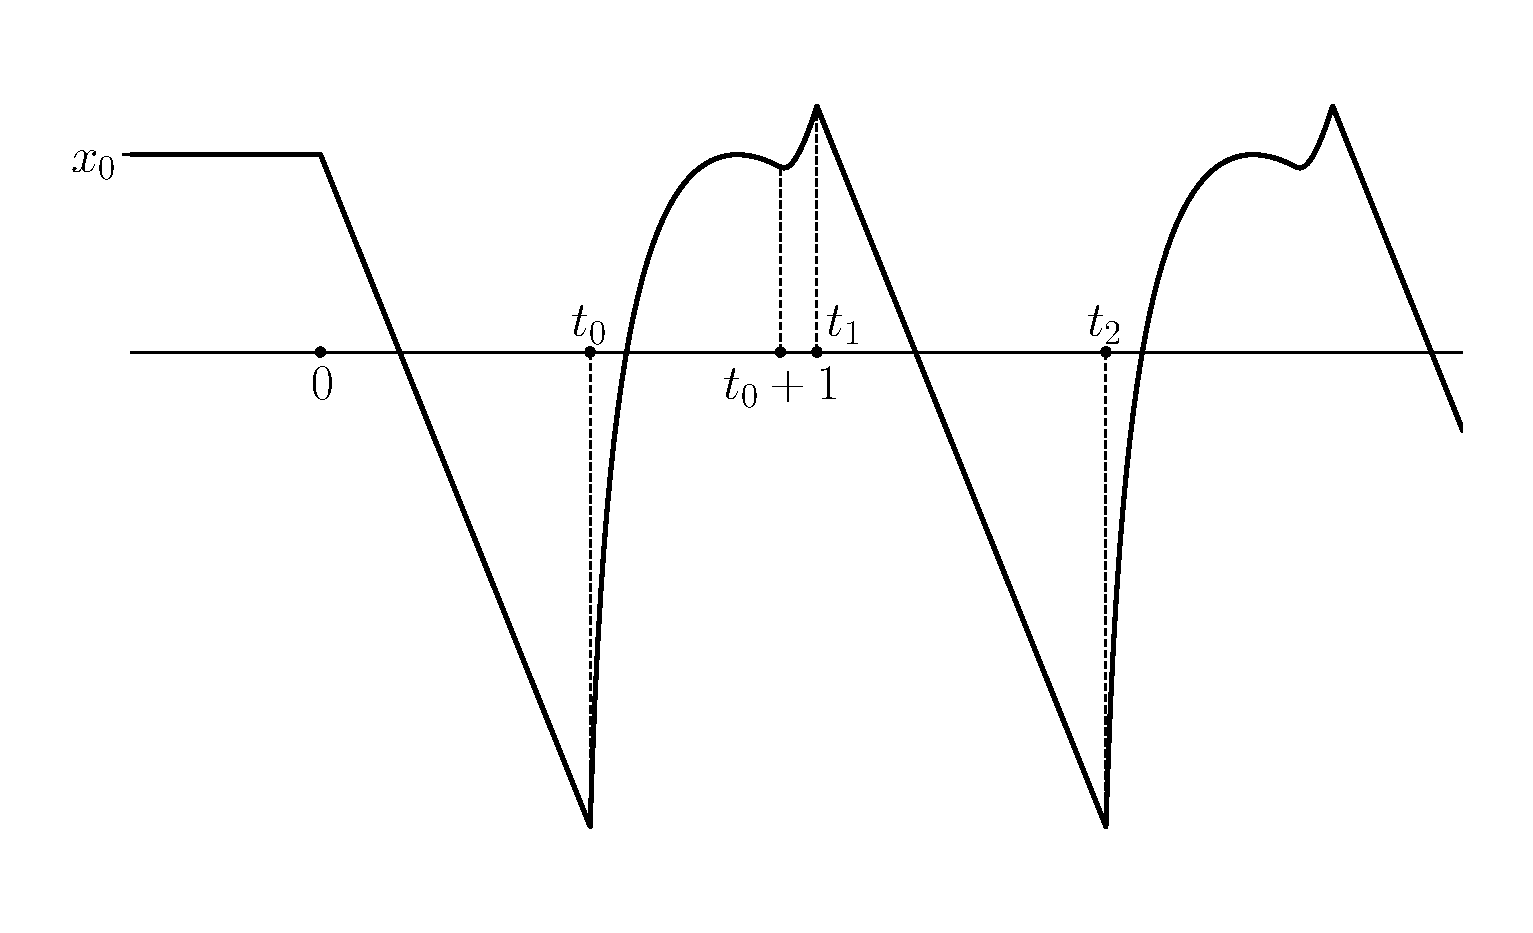
\includegraphics[width=0.7\textwidth]{x_star.eps}
	\captionof{figure}{The periodic solution $x^{*}(t)$ of equation \eqref{eq:intro:MG_rele}.}
	\label{fig:intro:x_star:ch1}
\end{figure}

Let us introduce auxiliary functions $w_i(\tau)$, $i = 0, 1$, to describe the solution in the neighborhoods of the points of discontinuity of the relay equation.
\[
w_i(\tau) = -\beta \tau - \dfrac{\alpha e^{-x^*(t_i)}}{\dot{x}^*(t_i - 1)} \ln\left(e^{-\dot{x}^*(t_i - 1)\tau} + 1\right) \quad \text{ for } \quad \dot{x}^*(t_i - 1) < 0,
\]
\[
w_i(\tau) = (-\beta + \alpha e^{-x^*(t_i)})\tau - \dfrac{\alpha e^{-x^*(t_i)}}{\dot{x}^*(t_i - 1)} \ln\left(e^{\dot{x}^*(t_i - 1)\tau} + 1\right) \quad \text{ for } \quad \dot{x}^*(t_i - 1) > 0,
\]
The corresponding values of the function $x^*(t)$ are obtained from the formulas \eqref{eq:intro:sol_x_star}.

The given functions satisfy asymptotic properties.

If $\dot{x}^*(t_i - 1) < 0$,
\begin{equation*}
	w_i(\tau) = -\beta \tau + O(\exp(-\dot{x}^*(t_i - 1) \tau)) \text{ for } \tau \to -\infty,
\end{equation*}
\begin{equation*}
	w_i(\tau) = (-\beta + \alpha e^{-x^*(t_i)})\tau + O(\exp(\dot{x}^*(t_i - 1) \tau)) \text{ for } \tau \to +\infty.
\end{equation*}

If $\dot{x}^*(t_i - 1) > 0$,
\begin{equation*}
	w_i(\tau) = (-\beta + \alpha e^{-x^*(t_i)})\tau + O(\exp(\dot{x}^*(t_i - 1) \tau)) \text{ при } \tau \to -\infty,
\end{equation*}
\begin{equation*}
	w_i(\tau) = -\beta \tau + O(\exp(-\dot{x}^*(t_i - 1) \tau)) \text{ при } \tau \to +\infty.
\end{equation*}

The coefficients of $\tau$ in the provided formulas coincide with the one-sided derivatives at the points of discontinuity of the solution to the relay equation $t_i$ for $i = 0, 1$.

The main result of the chapter is formulated as follows.

\bigskip

\textbf{Theorem.} \textit{Let the parameters $\alpha > \beta > 0$ satisfy conditions \eqref{eq:intro:cond_alpha1}, \eqref{eq:intro:cond_alpha2}. Then there exist values of the parameters $\sigma_0, p, q$ and a sufficiently large $\gamma_0$, such that for all $\gamma > \gamma_0$ equation \eqref{eq:intro:MG_x} with the initial function $\varphi$ from the set \eqref{eq:intro:init_set} has a periodic solution $x^*_\gamma(t, \varphi)$ with period $T_{\gamma, \varphi}$ and asymptotic}
\footnotesize
\begin{equation}
	\label{eq:intro:sol_x*gamma}
	x^*_\gamma(t, \varphi)= 
	\begin{cases}
		- \beta t + O(\gamma^{-1} e^{-\beta \delta \gamma}), & t\in[-\sigma_0, 1 - \delta],\\
		-\beta + \frac{1}{\gamma} w_0(\tau)|_{\tau=(t - 1)\gamma} + O(\gamma^{-2\nu}), & t \in [1 - \delta,1 + \delta],\\
		- \beta t + \ln(\alpha e^{\beta}(t - 1) + 1) + O(\gamma^{-2\nu}) & t\in[1 + \delta, 2]\\
		- \beta t + \ln(\frac{\alpha^2}{2}e^{2 \beta}(t - 2)^2 + \alpha e^{\beta}(t - 1) + 1) + O(\gamma^{-2\nu}), & t \in [2, t_1 - \delta],\\
		- \beta t_1 + \ln(\eta)+\frac{1}{\gamma} w_1(\tau)|_{\tau=(t - t_1)\gamma} + O(\gamma^{-2\nu}), & t\in[t_1 - \delta, t_1  +\delta],\\
		- \beta t + \ln(\eta) + O(\gamma^{-2\nu}), & t \in [t_1 + \delta, t_2 - \delta],
	\end{cases}
\end{equation}
\normalsize
where $\nu \in (\frac{1}{2}, 1)$, $\delta = \gamma^{-\nu}$, $\eta=\frac{\alpha^2}{2}e^{2\beta}(t_1 - 2)^2 + \alpha e^{\beta}(t_1 - 1) + 1$.
%
\textit{The given solution satisfies the limiting equalities}
%
\begin{equation}
	\label{eq:intro:lim_x*}
	\lim_{\gamma\to+\infty}\max_{0\leqslant t\leqslant T_{\gamma, \varphi}}|x_{\gamma}^*(t, \phi)-x^*(t)|=0,\quad \lim_{\gamma\to+\infty}T_{\gamma, \varphi} = T.
\end{equation}
\textit{All remainders and limits are uniform with respect to $\varphi \in S$ and $t$ from the corresponding intervals.}

\pdfbookmark{Content of the second chapter}{chsecond}
\textbf{Content of the second chapter.} In the second chapter, a fully connected network of relay oscillators described by the system \eqref{eq:intro:mg_full_renormed} is considered. We will look for a solution in the form of a discrete traveling wave. After substituting $u_j(t) = u(t + j\Delta)$, we obtain the auxiliary equation \eqref{eq:intro:mg_auxiliary}.

We normalize the time so that the smallest delay in the auxiliary equation becomes equal to 1. Let $1 = \tau_0 \leq \tau_1 \leq \ldots \leq \tau_N$ be the set of delays after normalization. We obtain the equation
\begin{equation}
	\label{eq:intro:mg_relay_w}
	\dot{u}=-\beta u+\alpha F(w(t)), \text{ where } w(t) = \sum\limits_{s = 0}^N u(t - \tau_s).
\end{equation}
%
Let us define the set of initial functions over the interval of the length of the largest delay: 
%
\begin{equation}
	\label{eq:intro:mg_init_set}
	\{\varphi\in C[-\tau_{N},0]:\  \varphi(t)>1 \text{ for } t\in[-\tau_{N},0),\ \varphi(0)=u_0 > 1\}.
\end{equation}
%
Introduce the notation:
%
\begin{equation*}
	A = \sum_{i=0}^{m}e^{\beta \tau_{i}}=e^\beta+e^{\beta \tau_1}+\ldots+e^{\beta \tau_{N}},
\end{equation*}
\begin{equation*}
	\tau_* = \min\{2,\tau_1\}=\left\lbrace\begin{array}{cl}
		\min\{2,1/\Delta\}, & \text{ if } \Delta < 1,
		\\
		\min\{2,\Delta\}, & \text{ if } \Delta > 1,
	\end{array}\right.
\end{equation*}
\begin{equation*}
	s_* = t_1-t_0.
\end{equation*}
%
For the auxiliary equation \eqref{eq:intro:mg_relay_w}, the following theorem has been proven.

\textbf{Theorem.} \textit{Let the parameters $\alpha, \beta, \tau_*$ satisfy the constraints}

\begin{equation}
	\label{eq:intro:cond_thm1}
	\frac{\alpha}{\beta}e^{\beta}\left(\ln\left(\frac{\beta}{\alpha}\right)+1\right) < 1,
	\quad
	\alpha > \beta.
\end{equation}
%
\begin{equation}
	\label{eq:intro:cond_thm2}
	e^{\beta \tau_*}-1 \leqslant \alpha e^\beta(\tau_*-1)
	\quad\text{ or }\quad
	0 < \frac{1}{\beta}\ln\frac{\alpha}{\beta}\leqslant\tau_*-1,
\end{equation}
%
\begin{equation}
	\label{eq:intro:cond_th_w>1_t_1+1}
	e^{-\beta s_*}(e^{-\beta}+\alpha s_*)>1
\end{equation}
%
\begin{equation}
	\label{eq:intro:cond_hair_hair_01}
	\frac{\alpha^2}{2}e^\beta(s_*-1)^2+\alpha s_*>\frac{e^{\beta \tau_k}-1}{\sum_{i=0}^{k-1}e^{\beta \tau_i}},\text{ if } s_*\leqslant \tau_k-\tau_{k-1},\quad k=1,\ldots,N,
\end{equation}
%
\begin{equation}
	\label{eq:intro:cond_hair_hair_02}
	\frac{\alpha^2}{2}e^\beta(s_*-1)^2+\alpha s_*>\frac{e^{\beta (s_*+\tau_{k-1})}-1}{\sum_{i=0}^{k-1}e^{\beta \tau_i}},\text{ if } s_* > \tau_k-\tau_{k-1},\quad k=1,\ldots,N,
\end{equation}
%
\begin{equation}
	\label{eq:intro:cond_hair_hair_1}
	\frac{\alpha^2}{2}e^\beta( s_*-1)^2+\alpha s_*>\frac{(e^{\beta s_*}-\alpha s_*)e^{\beta \tau_k}-1}{\sum_{i=0}^{k-1}e^{\beta \tau_i}},\quad k=1,\ldots,N.
\end{equation}
\textit{Then the solution of equation \eqref{eq:intro:mg_relay_w} for any initial function from the set \eqref{eq:intro:mg_init_set} coincides with the same periodic function. We will denote this function by $u_*$ and its period by $T$. The following holds true.}

\textit{1. The function $u_*(t)$ has the smallest number of switches over the period: $t_0$, $t_1$. Moreover, }
%
\begin{equation*}
	t_0=\frac{1}{\beta}\ln(u_0 A),
\end{equation*}
\begin{equation}
	e^{\beta s_*} - 1=\alpha e^{\beta}(s_* - 1), \quad s_* \in (1, \tau_*).
\end{equation}

\textit{2. The function $u_*(t)$ and the period $T$ have the following explicit form:}
%
\small
\begin{equation}
	\label{eq:intro:u_star}
	u_*(t)=
	\begin{cases}
		u_0 e^{-\beta t}(\alpha A(t-t_0)+1) & \text{ for } t\in[t_0,t_0+1].
		\\
		u_0 e^{-\beta t}\left(\frac{\alpha^2}{2}Ae^{\beta}(t-t_0-1)^2+\alpha A(t-t_0)+1\right) & \text{ for } t\in[t_0+1,t_1],
		\\
		u_0 e^{-\beta t}\left(\frac{\alpha^2}{2}Ae^{\beta}(t_1-t_0-1)^2+\alpha A(t_1-t_0)+1\right) & \text{ for } t\in[t_1,t_0+T].
	\end{cases}
\end{equation}
\normalsize
%
\[
u_*(t + T) \equiv u_*(t),
\]
%
\begin{equation}
	\label{eq:intro:mg_period_T}
	T = \dfrac{1}{\beta}\ln\left( \frac{\alpha^2}{2}Ae^{\beta}(t_1-t_0-1)^2+\alpha A(t_1-t_0)+1\right). 
\end{equation}
%
A schematic plot of the function $u_*$ is shown in the Fig. \ref{fig:intro:u_star}.
%
\begin{figure}[h]
	\centering
	\includegraphics[width=0.7\textwidth]{u_star_eng.eps}
	\caption{The function $u_*(t)$, defined over period $[t_0, t_0 + T]$ by the equation~\eqref{eq:intro:u_star}.}
	\label{fig:intro:u_star}
\end{figure}

To ensure the existence of a discrete traveling wave, it is necessary to verify that for some $\Delta$, the period of the solution to the auxiliary equation is a multiple of $\Delta (N + 1)$, where $(N + 1)$ is the number of equations in the system. That is, for some $p \in \mathbb{N}$, the following condition holds:
\begin{equation}
	\label{eq:intro:period_eq}
	pT = \Delta (N + 1).
\end{equation}

In the second chapter, the following theorem is proven.

\textbf{Theorem.} \textit{For arbitrary
	%
	\begin{equation}
		\label{eq:intro:constraints_parameters_final}
		\beta > 0, \alpha \geq e^{\beta\left(1 + \frac{1}{e^{\beta}}\right)} - 1
	\end{equation}
	%
	there exists $\Delta > 1$, such that the set of parameters $\alpha, \beta, \Delta$ satisfies equation \eqref{eq:intro:period_eq} for $p = 1$ and the conditions \eqref{eq:intro:cond_thm1}, \eqref{eq:intro:cond_thm2}, \eqref{eq:intro:cond_th_w>1_t_1+1}, \eqref{eq:intro:cond_hair_hair_01}, \eqref{eq:intro:cond_hair_hair_02}, \eqref{eq:intro:cond_hair_hair_1}.}
	
From the validity of this theorem, it immediately follows the existence of a solution in the form of a discrete traveling wave for the system \eqref{eq:intro:mg_full_renormed} under the given constraints on the parameters. Numerical experiments indicate that the solution is stable; moreover, the results of the experiments suggest the global attractivity of solutions of this type.

\bigskip

\pdfbookmark{Content of the third chapter}{third}
\textbf{Content of the third chapter.} In the third chapter, a fully coupled network consisting of $N = m + n$ relay oscillators of Mackey--Glass is considered; it described by the system \eqref{eq:intro:mg_full_renormed_delta}. We will look for a solution that describes the mode of two-cluster synchronization. After substituting \eqref{eq:intro:cluster}, we obtain the auxiliary system \eqref{eq:intro:system_uv}.

After substituting
\begin{equation}
	\label{eq:intro:tilde_change}
	\tilde{u}(t) = u(t - 1) + \delta (m - 1) u + \delta n v, \quad \tilde{v}(t) = v(t - 1) + \delta m u + \delta (n - 1) v
\end{equation}
%
and the subsequent exponential substitution
\begin{equation}
	\label{eq:intro:exp_change}
	\tilde{u} = e^x, \quad \tilde{v} = e^y
\end{equation}
%
the system \eqref{eq:intro:system_uv} takes the form
%
\begin{equation}
	\label{eq:intro:system_cluster_main}
	\begin{cases}
		\dot{x} = -\beta + \alpha \left(e^{x(t - 1) - x} G_{\gamma} (x(t - 1)) + \delta (m - 1) G_{\gamma} (x) + \delta n e^{y - x} G_{\gamma} (y)\right),\\
		\dot{y} = -\beta + \alpha \left(e^{y(t - 1) - y} G_{\gamma} (y(t - 1)) + \delta m e^{x - y} G_{\gamma} (x) + \delta (n - 1) G_{\gamma} (y)\right),
	\end{cases}
\end{equation}
where $G_{\gamma} (x) = e^{-x} \, F_{\gamma} (e^x)$.

The substitution \eqref{eq:intro:tilde_change} is valid in the sense of the following theorem.

\textbf{Theorem.} \textit{Let $(x, y)$ be a $T$-periodic solution of the system \eqref{eq:intro:system_cluster_main}. Then there exist $T$-periodic functions $u, v$, uniquely determined by the formulas \eqref{eq:intro:tilde_change}, \eqref{eq:intro:exp_change}, which are solutions of the system \eqref{eq:intro:system_uv}.}

As in the previous part of the dissertation, we will investigate the limiting object as $\gamma \to +\infty$. We will substitute the function $G_{\gamma} (x)$ by its limit version $G$:
\begin{equation}
	\label{eq:intro:relay_G_tilde}
	G(x) = \lim\limits_{\gamma \to +\infty} G_{\gamma}(x) = 
	\begin{cases}
		1, & x < 0,\\
		1/2, & x = 0,\\
		0, & x > 0.
	\end{cases}
\end{equation}
%
In this case, the right-hand side of the relay system \eqref{eq:intro:system_cluster_main} experiences a discontinuity at $x = 0$ and $y = 0$. An analysis of the system shows that its solution, upon reaching one of the discontinuity lines, can only continue along that line (transversal intersection with the discontinuity line is not possible).

We will construct the generalized solution using the method of equivalent control \cite[\S 4, p. 54]{Filippov1988}.

Consider the system
%
\small
\begin{equation}
	\label{eq:intro:system_main_relay}
	\begin{cases}
		\dot{x} = -\beta + \alpha \left(e^{x(t - 1) - x} g_x(x(t - 1), t - 1) + \delta (m - 1) g_x(x, t) + \delta n e^{y - x} g_y(y, t)\right),\\
		\dot{y} = -\beta + \alpha \left(e^{y(t - 1) - y} g_y(y(t - 1), t - 1) + \delta m e^{x - y} g_x(x, t) + \delta (n - 1) g_y(y, t)\right),\\
		g_x(x, t) = G(x) \quad\text{for } x \neq 0,\\
		g_y(y, t) = G(y) \quad\text{for } y \neq 0,
	\end{cases}
\end{equation}
\normalsize
%
where the functions $g_x(x, t)$ and $g_y(y, t)$ take values from the interval $(0, 1)$ when $x = 0$ (and similarly for $y = 0$), allowing the solution to continue along the line $x = 0$. As will be shown, the values of $g_x(0, t)$ and $g_y(0, t)$ at each step are uniquely determined from the equations $\dot{x} = 0$ and $\dot{y} = 0$, respectively. We will consider the functions $g_x$ and $g_y$ as part of the system.

The system \eqref{eq:intro:system_main_relay} will be referred to as a \emph{relay system}.

Let us define a family of pairs of initial functions on the interval $[-1, 0]$. Fix $x_0 > y_0 > 0$.
\begin{equation}
	\label{eq:intro:initial_set}
	S = \left\{(\phi, \psi) \in (C[-1, 0])^2 \,|\, \phi(t) > 0, \psi(t) > 0, x_0 = \phi(0), y_0 = \psi(0)\right\}.
\end{equation}

The following theorem has been proven.

\bigskip

\textbf{Theorem.}
\textit{Let}
%
\begin{equation}
	\label{eq:intro:constraint_1}
	x_0 - y_0 < \ln \dfrac{e^{2\beta}(n - \delta(n - 1)) - ne^{\beta} + \delta n(n - 1)}{\delta (n - 1)^2},
\end{equation}
\begin{equation}
	\label{eq:intro:constraint_2}
	\beta < \alpha \delta (m - 1), \quad \beta < \alpha \delta (n - 1),
\end{equation}
\small
\begin{equation}
	\label{eq:intro:constraint_3}
	e^{\beta} \cdot \dfrac{n - \delta(n - 1)}{\delta (n - 1)^2} > \dfrac{1}{n - 1} + \dfrac{1}{\delta(m - 1)}, \quad
	e^{\beta} \cdot \dfrac{m - \delta(m - 1)}{\delta (m - 1)^2} > \dfrac{1}{\delta(n - 1)} + \dfrac{1}{m - 1}.
\end{equation}
\normalsize

\textit{Under the constraints \eqref{eq:intro:constraint_1}, \eqref{eq:intro:constraint_2}, \eqref{eq:intro:constraint_3}, and for arbitrary initial functions from the set \eqref{eq:intro:initial_set}, the relay system \eqref{eq:intro:system_cluster_main} has a generalized solution described by the formulas}
%
\small
\begin{equation}
	\label{eq:intro:step1_solution}
	\begin{cases}
		x = x_0 - \beta t,\\
		y = y_0 - \beta t
	\end{cases}
	\textit{for } t \in [0, t_0], \textit{ where } t_0 = \dfrac{y_0}{\beta};
\end{equation}
%
\begin{equation}
	\label{eq:intro:step2_solution}
	\begin{cases}
		x = x_0 - \beta t + \ln\left(1 + \frac{n}{n - 1} e^{-x_0 + \beta t_0}  (e^{\beta  (t - t_0)} - 1)\right),\\
		y = 0,\\
		g_y(0, t) = \frac{\beta}{\alpha \delta (n - 1)}
	\end{cases}
	\textit{for } t \in [t_0, t_0 + 1];
\end{equation}
%
\begin{multline}
	\label{eq:intro:step3_solution}
	\begin{cases}
		x = -\beta t + \ln\left(\exp(x(t_{2i} + 1) + \beta (t_{2i} + 1)) + \frac{n (\delta(n - 1) - 1)}{\delta (n - 1)^2} (e^{\beta t} - \exp(\beta (t_{2i} + 1)))\right)
		,\\
		y = 0,\\
		g_y(0, t) = \frac{\beta}{\alpha} \cdot \frac{\delta (n - 1) - 1}{\delta^2 (n - 1)^2}
	\end{cases}\\
	\textit{for } t \in [t_{2i} + 1, t_{2i + 1}];
\end{multline}
%
\begin{multline}
	\label{eq:intro:step4_solution}
	\begin{cases}
		x = 0,\\
		y = -\beta t + \ln\left(\exp(\beta t_{2i + 1}) + \left(\frac{1}{\delta(n - 1)} + \frac{m}{m - 1}\right) (e^{\beta t} - \exp(\beta t_{2i + 1}))\right),\\
		g_x(0, t) = \frac{\beta}{\alpha \delta (m - 1)}
	\end{cases}\\
	\textit{for } t \in [t_{2i + 1}, t_{2i} + 2];
\end{multline}
%
\begin{multline}
	\label{eq:intro:step5_solution}
	\begin{cases}
		x = 0,\\
		y = -\beta t + \ln\left(\exp(y(t_{2i} + 2) + \beta (t_{2i} + 2)) + \left(\frac{\delta(n - 1) - 1}{\delta^2 (n - 1)^2} + \frac{m}{m - 1}\right) (e^{\beta t} - \exp(\beta (t_{2i} + 2)))\right),\\
		g_x(0, t) = \frac{\beta}{\alpha \delta (m - 1)}
	\end{cases}\\
	\textit{for } t \in [t_{2i} + 2, t_{2i + 1} + 1];
\end{multline}
%
\begin{multline}
	\label{eq:intro:step6_solution}
	\begin{cases}
		x = 0,\\
		y = -\beta t + \ln\left(\exp(y(t_{2i + 1} + 1) + \beta(t_{2i + 1} + 1)) + \frac{m (\delta (m - 1) - 1)}{\delta (m - 1)^2} (e^{\beta t} - \exp(\beta (t_{2i + 1} + 1))) \right),\\
		g_x(0, t) = \frac{\beta}{\alpha} \cdot \frac{\delta (m - 1) - 1}{\delta^2 (m - 1)^2}
	\end{cases}\\
	\textit{for } t \in [t_{2i + 1} + 1, t_{2i + 2}];
\end{multline}
%
\begin{multline}
	\label{eq:intro:step7_solution}
	\begin{cases}
		x = -\beta t + \ln\left(\exp(\beta t_{2i + 2}) + \left(\frac{1}{\delta(m - 1)} + \frac{n}{n - 1}\right) (e^{\beta t} - \exp(\beta t_{2i + 2}))\right),\\
		y = 0,\\
		g_y(0, t) = \frac{\beta}{\alpha \delta (n - 1)}
	\end{cases}\\
	\textit{for } t \in [t_{2i + 2}, t_{2i + 1} + 2];
\end{multline}
%
\begin{multline}
	\label{eq:intro:step8_solution}
	\begin{cases}
		x = -\beta t + \ln\left(\exp(x(t_{2i + 1} + 2) + \beta (t_{2i + 1} + 2)) + \left(\frac{\delta(m - 1) - 1}{\delta^2 (m - 1)^2} + \frac{n}{n - 1}\right) (e^{\beta t} - \exp(\beta (t_{2i + 1} + 2)))\right),\\
		y = 0,\\
		g_y(0, t) = \frac{\beta}{\alpha \delta (n - 1)}
	\end{cases}\\
	\textit{for } t \in [t_{2i + 1} + 2, t_{2i + 2} + 1];
\end{multline}
%
\begin{multline}
	\label{eq:intro:step9_solution}
	\begin{cases}
		x = -\beta t + \ln\left(\exp(y(t_{2i + 2} + 1) + \beta(t_{2i + 2} + 1)) + \frac{n (\delta(n - 1) - 1)}{\delta (n - 1)^2} (e^{\beta t} - \exp(\beta (t_{2i + 2} + 1))) \right),\\
		y = 0,\\
		g_y(0, t) = \frac{\beta}{\alpha} \cdot \frac{\delta (n - 1) - 1}{\delta^2 (n - 1)^2}
	\end{cases}\\
	\textit{for } t \in [t_{2i + 2} + 1, t_{2i + 3}].
\end{multline}
\normalsize
%	
\textit{Here, $i \geqslant 0$ is an integer. Each moment of time $t_{2i + 1}$ is defined as the root of the equation $x = 0$, where the function $x(t)$ is given by equation \eqref{eq:intro:step3_solution}. Each moment of time $t_{2i + 2}$ is defined as the root of the equation $y(t) = 0$, where the function $y(t)$ is determined from the system \eqref{eq:intro:step6_solution}. For all $i \geqslant 0$, it holds that $t_{i + 1} \in (t_i + 1, t_i + 2)$.}


\begin{figure}[!ht]
	\centering
	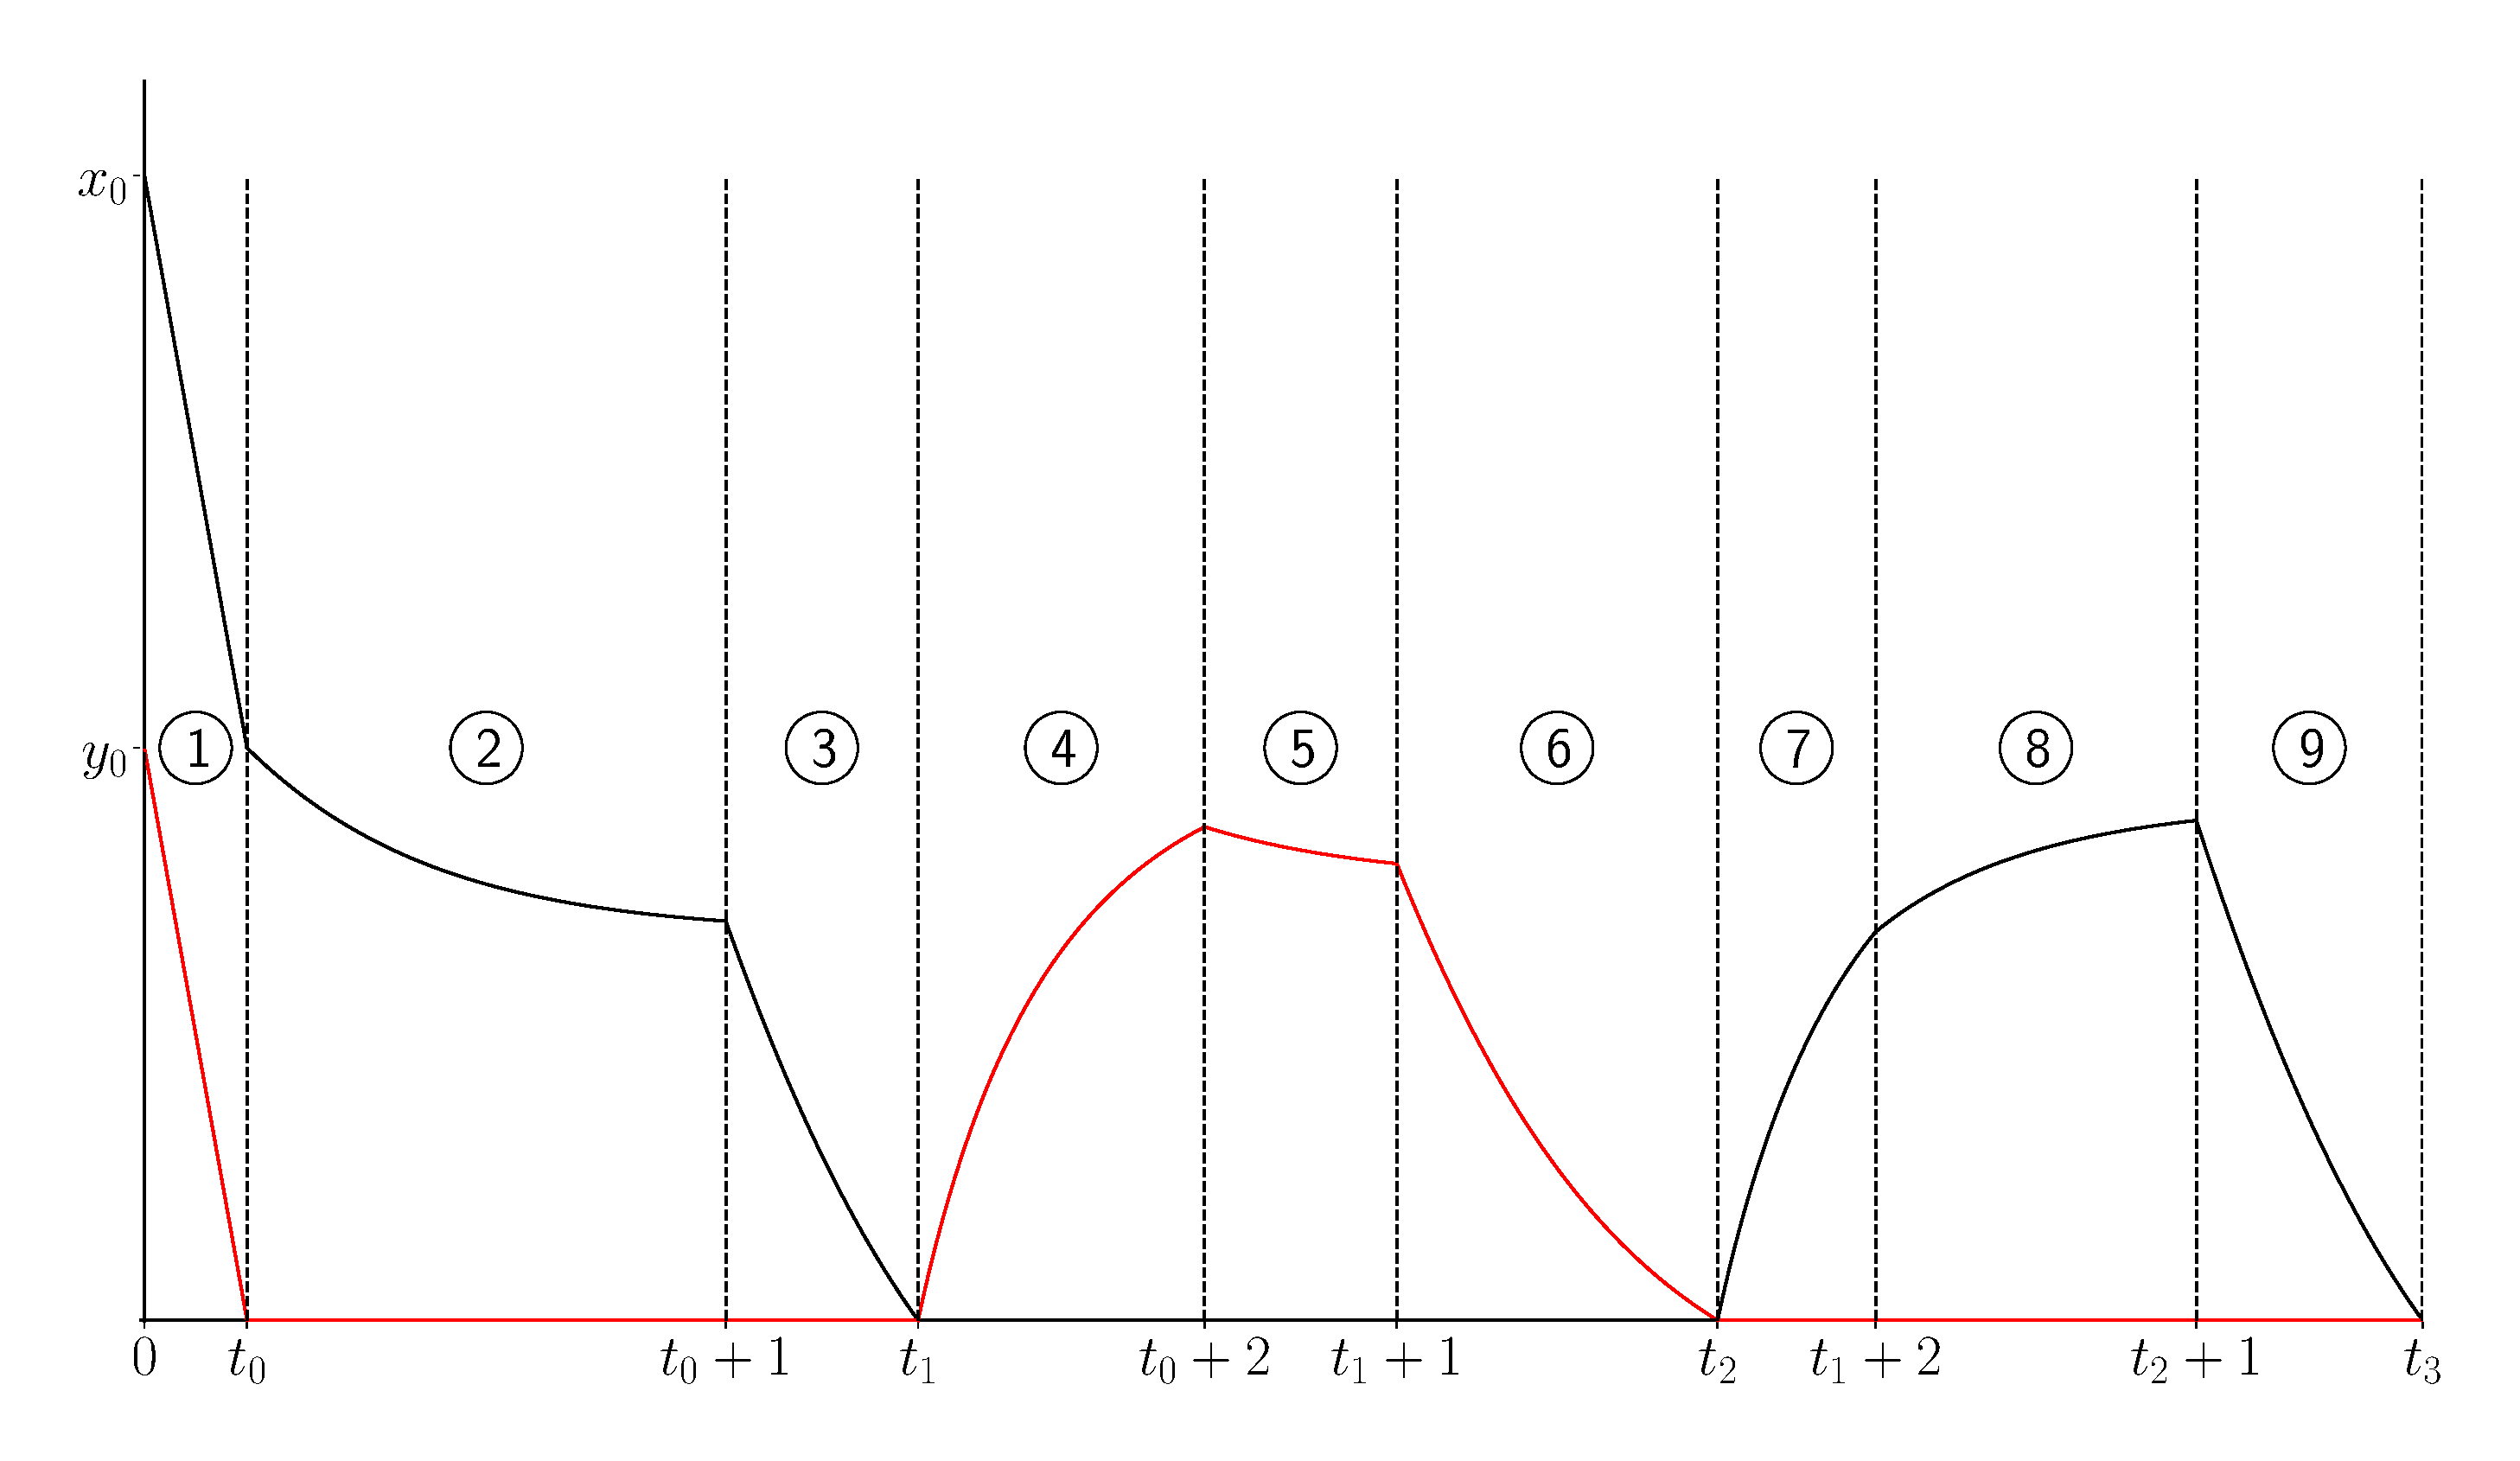
\includegraphics[width=\textwidth]{cluster_step_by_step.eps}
	\caption{The generalized solution of the relay system \eqref{eq:intro:system_cluster_main}, constructed using the method of steps. The black line represents the component of the solution $x$, the red line represents the component of the solution $y$. The numbers in the circles indicate the step number of the construction.}
	\label{fig:intro:cluster_step_by_step}
\end{figure}

The main result of the third chapter is the following theorem.

\textbf{Theorem.} \textit{Under the constraints \eqref{eq:intro:constraint_1}, \eqref{eq:intro:constraint_2}, \eqref{eq:intro:constraint_3} the relay system \eqref{eq:intro:system_cluster_main} has a periodic solution, described over the period $[t_1, t_3]$ by the formulas \eqref{eq:intro:step4_solution} -- \eqref{eq:intro:step9_solution}.}

\FloatBarrier
\pdfbookmark{Conclusion}{conclusion}                                  % Закладка pdf

The \textbf{conclusion} contains the main results of the work:
%% Согласно ГОСТ Р 7.0.11-2011:
%% 5.3.3 В заключении диссертации излагают итоги выполненного исследования, рекомендации, перспективы дальнейшей разработки темы.
%% 9.2.3 В заключении автореферата диссертации излагают итоги данного исследования, рекомендации и перспективы дальнейшей разработки темы.

\begin{enumerate}
  \item Asymptotic formulas for the periodic solution of the Mackey--Glass equation have been obtained for sufficiently large values of the nonlinearity coefficient. It has been shown that the asymptotic relations imply the convergence of the solution of the Mackey--Glass equation to the solution of the corresponding limiting relay equation.
  \item Sufficient conditions for the existence of periodic modes have been formulated and proven: (a) in the form of a discrete traveling wave, and (b) of two-cluster synchronization in a fully coupled network of Mackey--Glass relay oscillators, expressed as constraints on the parameters of the corresponding system of differential equations with delays.
  \item Numerical modeling of a fully connected network of Mackey--Glass relay oscillators has been conducted, suggesting the stability of the modes of discrete traveling waves and cluster synchronization.
\end{enumerate}


\pdfbookmark{Bibliography}{bibliography}                               % Закладка pdf

\renewcommand*{\insertbiblioauthor}{
	\printbibliography[heading=pubgroup, section=0, filter=papersregistered, title=\bibtitleauthorEng]
}

\renewcommand*{\insertbiblioexternal}{
	\printbibliography[heading=pubgroup,    section=0, keyword=biblioexternal, title=\bibtitlefullEng]
}

\ifdefmacro{\microtypesetup}{\microtypesetup{protrusion=false}}{} % не рекомендуется forменять пакет микротипографики к автоматически генерируемому списку литературы
\urlstyle{rm}                               % ссылки URL обычным шрифтом
\ifnumequal{\value{bibliosel}}{0}{% Встроенная реализация с загрузкой файла через движок bibtex8
    \renewcommand{\bibname}{\large \bibtitleauthorEng}
    \nocite{*}
    \insertbiblioauthor           % Подключаем Bib-базы
    %\insertbiblioexternal   % !!! bibtex не умеет работать с несколькими библиографиями !!!
}{% Реализация пакетом biblatex через движок biber
    % Цитирования.
    %  * Порядок перечисления определяет порядок в библиографии (только внутри подраздела, если `\insertbiblioauthorgrouped`).
    %  * Если не соблюдать порядок "как для \printbibliography", нумерация в `\insertbiblioauthor` будет кривой.
    %  * Если цитировать каждый источник отдельной командой --- найти некоторые ошибки будет проще.
    %
    %% authorvak
    \nocite{vakbib1}%
    \nocite{vakbib2}%
    %
    %% authorwos
    \nocite{wosbib1}%
    %
    %% authorscopus
    \nocite{scbib1}%
    %
    %% authorpathent
    \nocite{patbib1}%
    %
    %% authorprogram
    \nocite{progbib1}%
    %
    %% authorconf
    \nocite{confbib1}%
    \nocite{confbib2}%
    %
    %% authorother
    \nocite{bib1}%
    \nocite{bib2}%

    \ifnumgreater{\value{usefootcite}}{0}{
        \begin{refcontext}[labelprefix={}]
            \ifnum \value{bibgrouped}>0
                \insertbiblioauthorgrouped    % Вывод всех работ автора, сгруппированных по источникам
            \else
                \insertbiblioauthor      % Вывод всех работ автора
            \fi
        \end{refcontext}
    }{
        \ifnum \totvalue{citeexternal}>0
            \begin{refcontext}[labelprefix=A]
                \ifnum \value{bibgrouped}>0
                    \insertbiblioauthorgrouped    % Вывод всех работ автора, сгруппированных по источникам
                \else
                    \insertbiblioauthor      % Вывод всех работ автора
                \fi
            \end{refcontext}
        \else
            \ifnum \value{bibgrouped}>0
                \insertbiblioauthorgrouped    % Вывод всех работ автора, сгруппированных по источникам
            \else
                \insertbiblioauthor      % Вывод всех работ автора
            \fi
        \fi
        %  \insertbiblioauthorimportant  % Вывод наиболее значимых работ автора (определяется в файле characteristic во второй section)
        \begin{refcontext}[labelprefix={}]
            \insertbiblioexternal            % Вывод списка литературы, на которую ссылались в тексте автореферата
        \end{refcontext}
        % Невидимый библиографический список для подсчёта количества внешних публикаций
        % Используется, чтобы убрать forставку "А" у работ автора, если в автореферате нет
        % цитирований внешних источников.
        \printbibliography[heading=nobibheading, section=0, env=countexternal, keyword=biblioexternal, resetnumbers=true]%
    }
}
\ifdefmacro{\microtypesetup}{\microtypesetup{protrusion=true}}{}
\urlstyle{tt}                               % возвращаем установки шрифта ссылок URL
  % Содержание автореферата
%\clearpage                                  % В том числе гарантирует, что список литературы в оглавлении будет с правильным номером страницы
%\hypersetup{ urlcolor=black }               % Ссылки делаем чёрными
%\providecommand*{\BibDash}{}                % В стилях ugost2008 отключаем использование тире как разделителя
\urlstyle{rm}                               % ссылки URL обычным шрифтом
\ifdefmacro{\microtypesetup}{\microtypesetup{protrusion=false}}{} % не рекомендуется применять пакет микротипографики к автоматически генерируемому списку литературы
%\insertbibliofull                           % Подключаем Bib-базы: все статьи единым списком
% Режим с подсписками
\insertbiblioexternal                      % Подключаем Bib-базы: статьи, не являющиеся статьями автора по теме диссертации
% Для вывода выберите и расскомментируйте одно из двух
%\insertbiblioauthor                        % Подключаем Bib-базы: работы автора единым списком 
\insertbiblioauthorgrouped                 % Подключаем Bib-базы: работы автора сгруппированные (ВАК, WoS, Scopus и т.д.)
\ifdefmacro{\microtypesetup}{\microtypesetup{protrusion=true}}{}
\urlstyle{tt}                               % возвращаем установки шрифта ссылок URL
%\hypersetup{ urlcolor={urlcolor} }          % Восстанавливаем цвет ссылок
      % Список литературы

%%% Выходные сведения типографии
%\newpage\thispagestyle{empty}

%\vspace*{0pt plus1fill}

%\small
%\begin{center}
%    \textit{\thesisAuthor}
%    \par\medskip
%
%    \thesisTitle
%    \par\medskip
%
%    Автореф. дис. на соискание ученой степени \thesisDegreeShort
%    \par\bigskip
%
%    Подписано в печать \blank[\widthof{999}].\blank[\widthof{999}].\blank[\widthof{99999}].
%    Заказ № \blank[\widthof{999999999999}]
%
%    Формат 60\(\times\)90/16. Усл. печ. л. 1. Тираж 100 экз.
%    %Это не совсем формат А5, но наиболее близкий, подробнее: http://ru.wikipedia.org/w/index.php?oldid=78976454
%
%    Типография \blank[0.5\linewidth]
%\end{center}
%\cleardoublepage

\end{document}
